\documentclass[titlepage]{article}
\usepackage{xcolor}
\usepackage[english, croatian]{babel}

\usepackage{verbatim}
\usepackage{graphicx}
\usepackage{float}
\graphicspath{ {./Dijagrami_slike/} }

\title{INFORMACIONI SISTEMI\\Kovid sistem}
\author{
Bogdan Bojović 1019/2021\\
Kosta Grujčić 1012/2021\\
Miodrag Radojević 1012/2020\\
Luka Đorović 1029/2021\\
Irena Vasiljević 1018/2021
}

\date{Beograd, 2021.}

\begin{document}

\maketitle
\tableofcontents

\newpage

\section{Uvod}

\section{Analiza sistema}
Informacioni sistem Kovid centar svojim funkcionalnostima obezbe\dj{}uje sigurno i jednostavno sprovo\dj{}enje procedura neophodnih za za\v{s}titu od virusa COVID-19. \newline
\noindent Pored manipulacije podacima o testiranim i vakcinisanim pacijentima, informacioni sistem mehanizmima registracije i prijave pacijenatima pru\v{z}a mogu\'{c}nost automatizacije dodeljivanja termina vakcinacije i obave\v{s}tavanje o istim. Omogu\'{c}eno je  izdavanje i validacija kovid propusnice koja predstavlja garanciju da vlasnik ne predstavlja pretnju za suzbijanje virusa. Bitan deo predstavlja saradnja sa ministarstvom zdravlja, koja uklju\v{c}uje bezbedno dostavljanje relevantnih podataka ministarstvu. Komunikacija de\v{z}urnog medicinskog radnika sa pacijentom realizovana je posredstvom Kol centra, gde se pacijenti mogu detaljinije informisati o virusu ili  posavetovati u slu\v{c}aju prisustva nekih tegoba, nakon čega informacije o simptomima i tegobama bivaju čuvane u sistemu i biće dostupne ministarstvu zdravlja za dalje razmatranje.\newline
\indent Na Slici \ref{slk:slucajevi} nalazi se dijagram koji prikazuje učesnike sistema i njihove poslove. Slika \ref{slk:kontekst} prikazuje dijagram interakcije sistema sa svetom, a na Slici \ref{slk:dtp} se nalazi dijagram koji opisuje glavne procese i tok podataka u sistemu.

\begin{figure}[H]
\centering
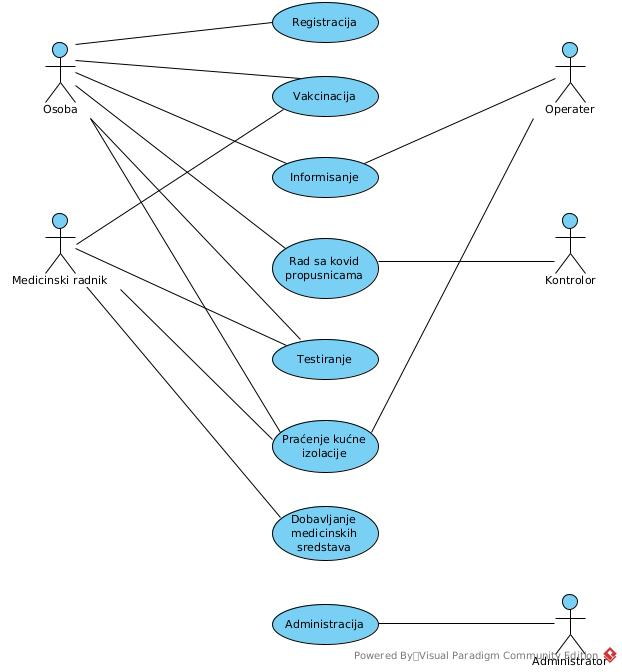
\includegraphics[scale=0.6]{Dijagram_slucajeva_upotrebe}
\caption{Dijagram slučajeva upotrebe}
\label{slk:slucajevi}
\end{figure}

\begin{figure}[H]
\centering
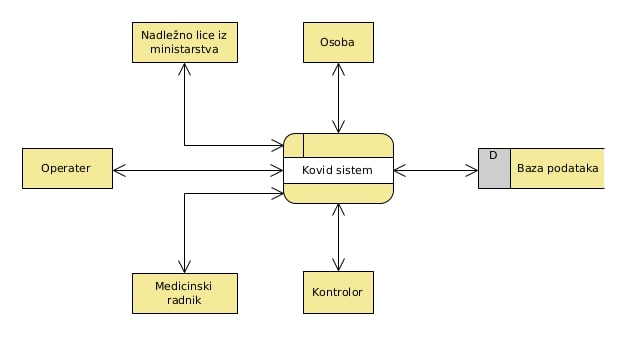
\includegraphics[scale=0.6]{Dijagram_konteksta}
\caption{Dijagram konteksta}
\label{slk:kontekst}
\end{figure}

\begin{figure}[H]
\centering
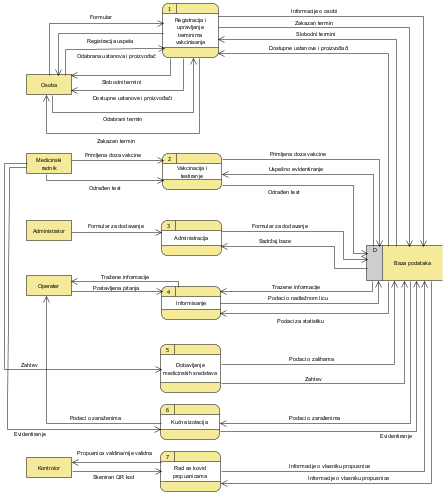
\includegraphics[scale=0.6]{DTP_dijagram}
\caption{Dijagram toka podataka nivoa 0}
\label{slk:dtp}
\end{figure}


\section{Procesi i slučajevi upotrebe}

%Menjajte strukturu i nazive kako vam se uklapa u slučaj :)

\subsection{Registracija}

\subsubsection{Slučaj upotrebe: Online registracija}
\begin{itemize}
    \item \textbf{Kratak opis:} Neregistrovana osoba vrši registraciju popunjavanjem online forme, traženim podacima. Sistem potvrđuje validnost podataka i vraća potvrdu o uspešnosti registracije.
    \item \textbf{Učesnici:}
        \begin{itemize}
            \item Neregistrovana osoba - želi da se registruje u sistem, u cilju podnošenja zahteva za vakcinaciju.
        \end{itemize}
    \item \textbf{Preduslovi:} Sistem je aktivan. Neregistrovana osoba ima pristup internetu.
    \item \textbf{Postuslovi:} Osoba je registrovana i ima pristup sistemu. Njeni podaci su sačuvani u bazi. Dobila je korisničko ime i lozinku uz pomoć kojih se loguje na sistem.
    \item \textbf{Osnovni tok:}
        \begin{enumerate}
            \item Osoba otvara web-stranicu za registraciju.
	    \item Sistem prikazuje formular za registraciju.
	    \item Osoba unosi tražene podatke.
	    \item Osoba potvrđuje unos.
	    \item Sistem vrši validaciju podataka.
	    \item Sistem čuva podatke.
	    \item Sistem pravi privremeni nalog.
	    \item Sistem šalje osobi email u kojem traži potvrdu registracije.
	    \item Sistem obaveštava osobu da je email poslat.
	    \item Osoba proverava poštu i potvrđuje registraciju.
	    \item Sistem privremeni nalog trajno aktivira.
            \item Sistem obaveštava osobu da je uspešno registrovana.
	\end{enumerate}
     
    %Ako postoje, podtokove nazivati sa P1, P2, ...   
    %\item \textbf{Podtokovi:}    
    
    %Alternativne tokove nazivati sa A1, A2, ...
    \item \textbf{Alternativni tokovi:}
        \begin{itemize}
            \item[A1.] \textbf{Neuspešna validacija podataka.} Ukoliko u koraku 5 osnovnog toka sistem naiđe na neispravne podatke, obaveštava korisnika i zahteva ponovni unos onih polja gde su nevalidni podaci. Pri čemu označava korisniku polja sa nevalidnim podacima. Kada osoba unese sve podatke ispravno, proces se nastavlja u koraku 4 osnovnog toka.
            \item[A2.] \textbf{Nije stigao email za potvrdu registracije.} Ukoliko osoba nije dobila email za potvrdu, klikom na dugme zahteva ponovno slanje emaila. Proces se nastavlja u koraku 8.
	    \item[A3.] \textbf{Link za registraciju je istekao.} Ukoliko osoba nije potvrdila registraciju u predviđenom periodu, sistem briše privremeni nalog. Proces se završava.
        \end{itemize}
    
    %Ako postoje, specijalne zahteve navesti ovde
    \item \textbf{Specijalni zahtevi:}
		\begin{itemize}
			\item Potrebno je da je osoba koja se registruje punoletna.
		\end{itemize}
  
    \item \textbf{Dodatne informacije:}
        \begin{itemize}
            \item  Podaci potrebni za prijavu su:
                \begin{itemize}
                    \item ime
                    \item prezime
                    \item JMBG
                    \item broj zdravstvene knjižice
                    \item broj telefona
                    \item email adresa
		    \item korisničko ime
		    \item lozinka
                \end{itemize}
        \end{itemize}

\end{itemize}

\subsection{Vakcinacija}
Ovo poglavlje sačinjeno je od formalno predstavljenih slučajeva upotrebe počev od podnošenja prijave do evidentiranja uspešno primljene doze vakcine, kao i obaveštavanja o terminu primanja naredne doze.

\subsubsection{Slučaj upotrebe: Podnošenje prijave online}
\begin{itemize}
    \item \textbf{Kratak opis:} Neprijavljena osoba vrši prijavu popunjavanjem online forme, traženim podacima. Sistem potvrđuje validnost podataka i vraća poruku o uspešnosti prijave.
    \item \textbf{Učesnici:}
        \begin{itemize}
            \item Neprijavljena osoba - želi da se prijavi za prvu dozu vakcine.
        \end{itemize}
    \item \textbf{Preduslovi:} Sistem je aktivan. Neprijavljena osoba je registorvana kao korisnik sistema i ima pristup internetu.
    \item \textbf{Postuslovi:} Korisnik je dobio potvrdu o zakazanom terminu i mestu prve vakcinacije.
    \item \textbf{Osnovni tok:}
        \begin{enumerate}
            \item Osoba otvara web-stranicu za logovanje.
	    \item Osoba unosi i potvrđuje korisničko ime i lozinku.
            \item Sistem prikazuje formular za prijavu.
            \item Osoba bira ponuđene ustanove i proizvođače vakcina.
            \item Osoba potvrđuje unos.
            \item Sistem čuva unete podatke.
	    \item Sistem daje mogućnost izbora raspoloživih termina za zadate ustanove i vakcine.
	    \item Osoba bira ponuđene termine i potvrđuje. 
            \item Sistem zakazuje termin vakcinacije.
	    \item Sistem korisniku šalje email sa potvrdom o zakazanom terminu.
            \item Sistem obaveštava korisnika da je operacija uspešno izvršena i da je potvrda poslata.
	\end{enumerate}
     
    %Ako postoje, podtokove nazivati sa P1, P2, ...   
    %\item \textbf{Podtokovi:}    
    
    %Alternativne tokove nazivati sa A1, A2, ...
    \item \textbf{Alternativni tokovi:}
        \begin{itemize}
            \item[A1.] \textbf{Neuspešno logovanje.} Ukoliko u koraku 2 osnovnog toka sistem naiđe na neispravne podatke, obaveštava korisnika i zahteva ponovni unos korisničkog imena i lozinke. Proces se nastavlja u koraku 2 osnovnog toka.
        \end{itemize}
    
    %Ako postoje, specijalne zahteve navesti ovde
    \item \textbf{Specijalni zahtevi:}
		\begin{itemize}
			\item Potrebno je da je zdravstvena knjižica, osobe koja zakazuje vakcinaciju, u trenutku zakazivanja važeća.
		\end{itemize}
  
\end{itemize}

\begin{figure}[H]
\centering
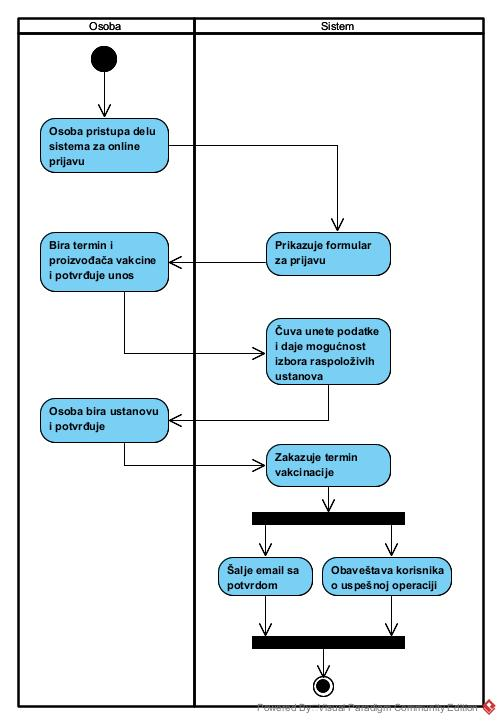
\includegraphics[scale=0.7]{Podnosenje_prijave_online}
\caption{Dijagram aktivnosti - Pondnošenje prijave online}
\end{figure}

\subsubsection{Slučaj upotrebe: Podnošenje prijave uživo}
\begin{itemize}
    \item \textbf{Kratak opis:} Neprijavljena osoba vrši prijavu popunjavanjem papirnog formulara, traženim podacima. Sistem potvrđuje validnost podataka i vraća poruku o uspešnosti prijave.
    \item \textbf{Učesnici:}
        \begin{itemize}
	    \item Medicinski radnik - pruža pomoć osobi u podnošenju prijave.
        %  \item Neprijavljena osoba - želi da se prijavi za prvu dozu vakcine.
	\end{itemize}
    \item \textbf{Preduslovi:} Sistem je aktivan.
    \item \textbf{Postuslovi:} Osoba je dobila potvrdu o zakazanom terminu i mestu prve vakcinacije.
    \item \textbf{Osnovni tok:}
        \begin{enumerate}
            \item Osoba dolazi na informacioni pult i izjavljuje da želi da se vakciniše.
	    \item Medicinski radnik na pultu odlazi na deo sistema koji je predviđen za registraciju novih korisnika.
	    \item Osoba daje potrebne informacije za registraciju, zdravstvenu knjižicu i neki lični dokument za evidenciju medicinskom radniku.
	    \item Medicinski radnik unosi podatke u sistem.
	    \item Medicinski radnik potvrđuje unos.
	    \item Sistem vrši validaciju podataka.
            \item Sistem čuva podatke.
            \item Sistem prikazuje informacije o nalogu koji kreira i traži potvrdu registracije.
	    \item Medicinski radnik nakon provere podataka potvrđuje registraciju osobe.
            \item Sistem obaveštava da je osoba uspešno registrovana.
	    \item Medicinski radnik od osobe traži da odabere ustanove i proizvođače vakcina.
	    \item Osoba obaveštava medicinskog radnika o odgovarajućim ustanovama i proizvođačima vakcine.
	    \item Medicinski radnik unosi podatke u sistem i potvrđuje.
	    \item Sistem dajte pregled slobodnih termina.
            \item Medicinski radnik obaveštava osobu o slobodnim terminima.
	    \item Osoba bira termin.
	    \item Medicinski radnik bira odgovarajući termin u sistemu i potvrđuje.
            \item Sistem zakazuje termin vakcinacije.
	    \item Sistem osobi šalje email sa potvrdom o zakazanom terminu.
            \item Sistem obaveštava medicinskog radnika da je operacija uspešno izvršena i da je potvrda poslata.
	    \item Medicinski radnik obaveštava osobu da je operacija uspešno izvršena i da je potvrda poslata na njen email.
	\end{enumerate}
     
    %Ako postoje, podtokove nazivati sa P1, P2, ...   
    %\item \textbf{Podtokovi:}    
    
    %Alternativne tokove nazivati sa A1, A2, ...
    \item \textbf{Alternativni tokovi:}
        \begin{itemize}
            \item[A1.] \textbf{Neuspešna validacija podataka.} Ukoliko u koraku 6 osnovnog toka sistem naiđe na neispravne podatke, obaveštava medicinskog radnika i zahteva ponovni unos onih polja gde su nevalidni podaci. Pri čemu označava polja sa nevalidnim podacima. Kada medicinski radnik unese sve podatke ispravno, proces se nastavlja u koraku 5 osnovnog toka.
	     \item[A2.] \textbf{Nema slobodnih termina.} Ukoliko u koraku 14 osnovnog toka medicinski radnik dobije obaveštenje od sistema da nema slobodnih termina za zadate ustanove i vakcine, on informaciju prenosi osobi i proces se nastavlja u koraku 11 osnovnog toka.
        \end{itemize}
    
    %Ako postoje, specijalne zahteve navesti ovde
    \item \textbf{Specijalni zahtevi:}
		\begin{itemize}
			\item Potrebno je da je zdravstvena knjižica, osobe koja zakazuje vakcinaciju, u trenutku zakazivanja važeća.
		\end{itemize}


     \item \textbf{Dodatne informacije:}
        \begin{itemize}
	    \item Dokument za evidenciju osobe čija se registracija vrši može biti pasoš ili lična karta.
            \item  Podaci potrebni za prijavu su:
                \begin{itemize}
                    \item ime
                    \item prezime
                    \item JMBG
                    \item broj zdravstvene knjižice
                    \item broj telefona
                    \item email adresa
		    \item korisničko ime
		    \item lozinka
                \end{itemize}
        \end{itemize}
  
\end{itemize}


\subsubsection{Slučaj upotrebe: Otkazivanje termina vakcinacije - online prijavljena osoba}
\begin{itemize}
    \item \textbf{Kratak opis:} Online prijavljena osoba za primanje prve doze vakcine, usled izvesnih okolnosti otkazuje zauzeti termin za primanje prve doze vakcine. Sistem potvrđuje odjavu i oslobađa termin.
    \item \textbf{Učesnici:}
        \begin{itemize}
            \item Prijavljena osoba - želi da se otkaže termin primanja prve doze vakcine.
        \end{itemize}
    \item \textbf{Preduslovi:} Sistem je aktivan. Osoba je prethodno zakazala primanje prve doze vakcine.
    \item \textbf{Postuslovi:} Osoba je dobila potvrdu o otkazanom terminu i ima mogućnost da se ponovo prijavi za primanje prve doze vakcine.
    \item \textbf{Osnovni tok:}
        \begin{enumerate}
            \item Osoba otvara web-stranicu za logovanje.
	    \item Osoba unosi i potvrđuje korisničko ime i lozinku.
	    \item Sistem prikazuje prethodno podnetu prijavu i informacije o njoj.
	    \item Osoba bira opciju za otkazivanje prijave i potvrđuje je.
	    \item Sistem otvara formu za unos razloga otkazivanja prijave.
	    \item Sistem zahteva od osobe da popuni formu.
	    \item Osoba unosi razlog otkazivanja prijave.
            \item Osoba potvrđuje unos razloga.
	    \item Sistem evidentira odjavu.
	    \item Sistem oslobađa termin za dato mesto, vakcinu i vreme.
	    \item Sistem osobi šalje email sa potvrdom o uspešnoj odjavi termina.
	    \item Sistem obaveštava osobu o uspešnoj odjavi termina i da je potvrda o odjavi poslata.
	\end{enumerate}
     
    %Ako postoje, podtokove nazivati sa P1, P2, ...   
    %\item \textbf{Podtokovi:}    
    
    %Ako postoje, specijalne zahteve navesti ovde
    \item \textbf{Specijalni zahtevi:}
		\begin{itemize}
			\item Potrebno je da osoba koja se odjavljuje ima validan razlog za otkazivanje prve primanja prve doze vakcine.
		\end{itemize}
\end{itemize}


\subsubsection{Slučaj upotrebe: Otkazivanje termina vakcinacije - uživo prijavljena osoba}
\begin{itemize}
    \item \textbf{Kratak opis:} Uživo prijavljena osoba za primanje prve doze vakcine, usled izvesnih okolnosti otkazuje zauzeti termin za primanje prve doze vakcine. Sistem potvrđuje odjavu i oslobađa termin.
    \item \textbf{Učesnici:}
        \begin{itemize}
	    \item Medicinski radnik - pruža pomoć osobi u podnošenju odjave.
              %   \item Prijavljena osoba - želi da se otkaže termin primanja prve doze vakcine.
	\end{itemize}
    \item \textbf{Preduslovi:} Sistem je aktivan. Osoba je prethodno zakazala primanje prve doze vakcine.
    \item \textbf{Postuslovi:} Osoba je dobila potvrdu o otkazanom terminu i ima mogućnost da se ponovo prijavi za primanje prve doze vakcine.
    \item \textbf{Osnovni tok:}
        \begin{enumerate}
            \item Osoba dolazi na informacioni pult ili telefonskim pozivom izjavljuje da želi da odjavi zauzeti termin.
	    \item Medicinski radnik na pultu odlazi na deo sistema koji je predviđen za odjavu prijavljenih osoba.
	    \item Sistem zahteva podatke osobe koja želi da odjavi termin.
	    \item Medicinski radnik zahteva podatke osobe koja se odjavljuje.
	    \item Osoba obaveštava medicinskog radnika o podacima.
	    \item Medicinski radnik unosi podatke u sistem i potvrđuje.
            \item Sistem za date podatke pronalazi registrovani nalog.
	    \item Sistem prikazuje nalog i prethodno zakazani termin.
	    \item Sistem zahteva unošenje razloga i potvrdu odjave.
	    \item Medicinski radnik proverava nalog osobe i prethodno zakazani termin.
	    \item Medicinski radnik zahteva razlog odjave termina od osobe.
	    \item Osoba obaveštava medicinskog radnika o razlogu odjave termina.
	    \item Medicinski radnik unosi razlog odjave termina i potvrđuje odjavu termina.
	    \item Sistem evidentira odjavu.
	    \item Sistem oslobađa termin za dato mesto, vakcinu i vreme.
	    \item Sistem obaveštava medicinskog radnika o uspešnoj odjavi termina.
	    \item Medicinski radnik obaveštava osobu o uspešnoj odjavi termina.
	\end{enumerate}
     
    %Ako postoje, podtokove nazivati sa P1, P2, ...   
    %\item \textbf{Podtokovi:}    
    
    %Alternativne tokove nazivati sa A1, A2, ...
    \item \textbf{Alternativni tokovi:}
        \begin{itemize}
            \item[A1.] \textbf{Nepostojeći podaci u bazi.} Ukoliko u koraku 7 osnovnog toka sistem za unete podatke ne pronađe nalog u bazi, obaveštava medicinskog radnika i zahteva ponovni unos podataka. Medicinski radnik obaveštava osobu o neispravnosti podataka i zahteva da se podaci ponovo daju. Proces se nastavlja u koraku 4 osnovnog toka.
        \end{itemize}
    
    %Ako postoje, specijalne zahteve navesti ovde
    \item \textbf{Specijalni zahtevi:}
		\begin{itemize}
			\item Potrebno je da osoba koja se odjavljuje ima validan razlog za otkazivanje prve primanja prve doze vakcine.
		\end{itemize}
\end{itemize}

\subsubsection{Slučaj upotrebe: Obaveštavanje o narednoj dozi vakcine}
\begin{itemize}
    \item \textbf{Kratak opis:} Sistem na osnovu podataka o primanju prethodne doze vakcine osobu prijavljuje za dobijanje naredne doze vakcine i obaveštava je o terminu.
    \item \textbf{Učesnici:} 
        \begin{itemize}
            \item Osoba - osoba koja treba da primi narednu dozu vakcine.
        \end{itemize}
    \item \textbf{Preduslovi:} Sistem je aktivan, podaci o vakcinaciji osobe su ažurni.
    \item \textbf{Postuslovi:} Osoba je prijavljena za dobijanje naredne doze vakcine i o tome biva obaveštena. Sistem je ažuriran.
    \item \textbf{Osnovni tok:}
    \begin{enumerate}
        \item Sistem pristupa podacima o vakcinisanima. Sistem ovu operaciju izvodi automatski, svakog dana u podne.
        \item Sistem predla\v{z}e vreme i mesto vakcinacije drugom dozom vakcine koja je već primljena prvi put.
        \item Osoba razmatra o vremenu i mestu vakcinacije.
        \begin{itemize}
            \item Osoba prihvata vreme i mesto vakcinacije.
            \item Osoba ne prihvata vreme i mesto vakcinacije.
        \end{itemize}
        \item 
        \begin{itemize}
            \item Ukoliko osoba prihvati vreme i mesto vakcinacije, izvršavanje se nastavlja u koraku 5 osnovnog toka.
            \item Ukoliko osoba ne prihvati vreme i mesto vakcinacije, izvršava se podtok P1.
        \end{itemize}
        \item Sistem a\v{z}urira podatke o zakazanim terminima.
        \item Sistem obave\v{s}tava osobu da je termin zakazan.
        
    \end{enumerate}
    \item \textbf{Podtokovi:}
    \begin{itemize}
        \item[P1.] Osoba ne prihvata termin vakcinacije. 
        \begin{enumerate}
        \item Sistem šalje formular osobi kako bi odabrala vreme i mesto vakcinacije
        \item Osoba upisuje vreme i mesto vakcinacije.
        \item Sistem validira unete podatke.
        \end{enumerate}
    \end{itemize}
    \item \textbf{Dodatne informacije:}
    \begin{itemize}
        \item Sistem treba ponuditi mogućnosti osobi koja želi da popuni formular, u vidu spiska lokacija Kovid-ambulanti i spiska dostupnih termina.
    \end{itemize}
\end{itemize}


\begin{figure}[H]
\centering
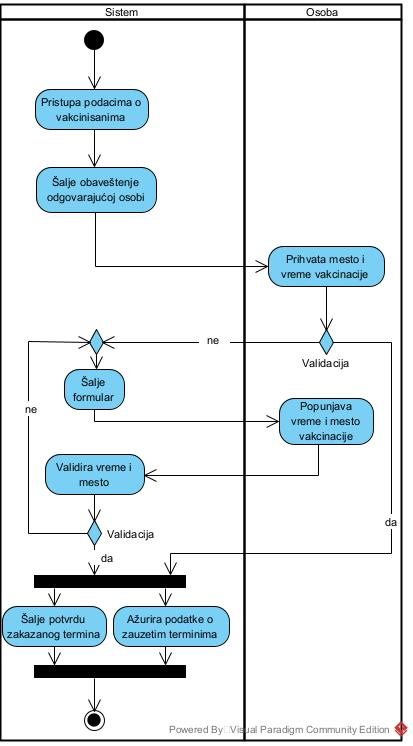
\includegraphics[scale=0.8]{Vakcinacija_drugom_dozom}
\caption{Dijagram aktivnosti - Obaveštavanje o narednoj dozi vakcine}
\end{figure}

\subsubsection{Slučaj upotrebe: Evidentiranje primljene doze}
\begin{itemize}
	\item \textbf{Kratak opis}: Osoba je prijavljena za vakcinaciju bilo kojom dozom. Nakon završene vakcinacije se sistem ažurira.
	\item \textbf{Učesnici}:
	\begin{itemize}
		\item Osoba - osoba koja se vaksiniše.
		\item Medicinski radnik - službeno lice koje vakciniše i upisuje potrebne informacije.
	\end{itemize}
	\item \textbf{Preduslovi}: Osoba ja prijavljena i ima zakazan termin. Sistem je aktivan.
	\item \textbf{Postuslovi}: Osoba je vaksinisana. Sistem je ažuriran.
	\item \textbf{Osnovni tok}:
	\begin{enumerate}
		\item Osoba medicinskom radniku daje svoju zdravstvenu knjižicu i ostale informacije potrebne za identifikaciju.
		\item Medicinski radnik proverava da li je osoba prijavljena za vakcinaciju.
		\item Osoba potpisuje saglasnost.
		\item Medicinski radnik vaksiniše osobu.
		\item Medicinski radnik evidentira da je osoba vakcinisana.
	\end{enumerate}
	\item \textbf{Alternativni tokovi}:
	\begin{enumerate}
		\item[A1.] Ako osoba ne želi da potpiše saglanost u koraku 3 osnovnog toga onda ona neće ni biti vakcinisana. 
	\end{enumerate}
\end{itemize}

\begin{center}
	\begin{figure}[H]
		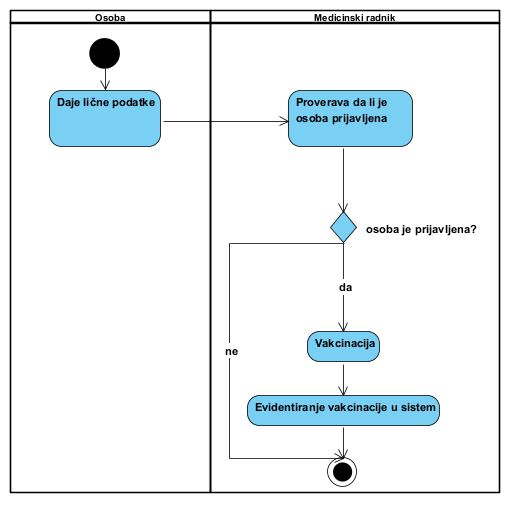
\includegraphics[width=0.95\textwidth]{Vakcinacija}
		\caption{Dijagram aktivnosti - Evidentiranje primljene doze}
	\end{figure}
\end{center}

\subsection{Informisanje}

U ovom poglavlju se bavimo predstavljanjem slučajeva upotrebe koji se tiču korišćenja našeg sistema radi informisanja.

\subsubsection{Slučaj upotrebe: Dodela specijalnog identifikacionog broja za dohvatanje statistike }
\begin{itemize}
    
\item \textbf{Kratak opis:} Ministarstvo zdravlja sistemu dostavlja podatke  o licima koja \'{c}e biti nadle\v{z}na za slanje zahteva za dohvatanje statistika dostupnih u informacionom sistemu. Nakon provere podataka, sistem za svako od odabranih lica vr\v{s}i registraciju na sistem i generi\v{s}e specijalni identifikacioni broj koji će se koristiti pri logovanju za podno\v{s}enje zahteva za dohvatanje statistike. 
\item \textbf{Učesnici:}
\begin{itemize}
    \item Nadle\v{z}no lice iz ministarstva zdravlja
\end{itemize}
 \item \textbf{Preduslovi:} Sistem je aktivan
 \item \textbf{Postuslovi:} Svakom od lica iz ministarstva koje je zadu\v{z}eno za dohvatanje statistike dostavljen je poseban identifikacioni broj koji će koristiti pri logovanju za slanje zahteva za dohvatanje statistike. 
 \item \textbf{Osnovni tok:}
 \begin{enumerate}
    \item Lice iz ministarstva zdravlja formira spisak nadle\v{z}nih lica za dohvatanje statistike.
    \item Taj spisak putem sigurnih kanala (bilo uživo bilo elektronski) biva dostavljen do informacionog sistema.
    \item Koriste\'{c}i posebne he\v{s} funkcije u pozadini, sistem generi\v{s}e identifikacione brojeve.
    \item Svaki od identifikacionih brojeva putem sigurnih kanala ( bilo u\v{z}ivo bilo elektronski) biva dostavljen svakom od lica iz ministarstva koje su se na\v{s}li na spisku nadle\v{z}nih za dohvatanje statistike.
    \item Svako od nadle\v{z}nih lica za dohvatanje statistike iz ministarstva zdravlja biva registrovano na sistem, i biva obave\v{s}teno da \'{c}e za logovanje na sistem za potrebe slanja zahteva za dohvatanje statistike koristiti dodeljen identifikacioni broj.
 \end{enumerate}
\end{itemize}

\begin{figure}[H]
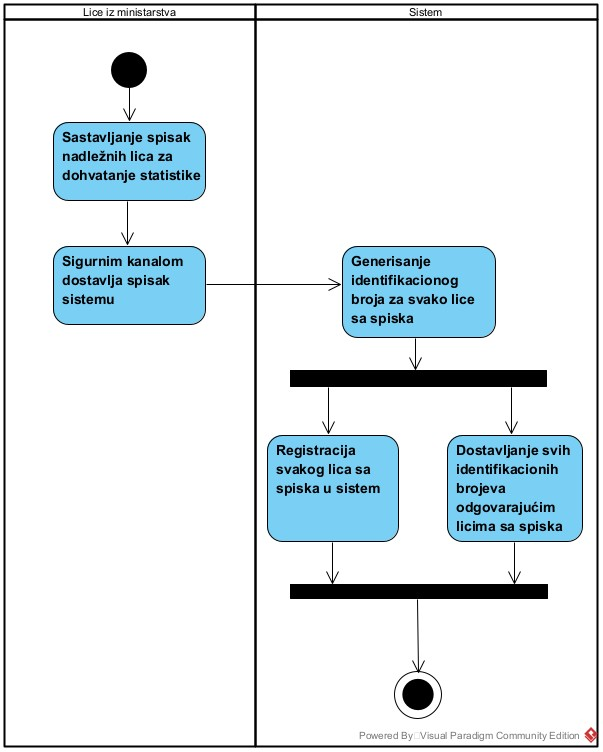
\includegraphics[scale=0.53]{Dodela_ID_za_dohvatanje_statistike.jpg}
\caption{Dijagram aktivnosti - Sprovo\dj{}enje statistike nadle\v{z}nom licu}
\end{figure}

\subsubsection{Slučaj upotrebe: Sprovođenje statistike nadle\v{z}nom licu}
\begin{itemize}
\item \textbf{Kratak opis:}  Nadle\v{z}no lice iz ministarstva zdravlja popunjava formular na osnovu kojeg mu se nakon autentikacije i konsultovanja baze podataka u malom broju koraka dostavljaju tra\v{z}eni podaci.
\item \textbf{Učesnici:}
\begin{itemize}
    \item Nadle\v{z}no lice iz ministarstva iz zdravlja.
\end{itemize}
 \item \textbf{Preduslovi:} Sistem je aktivan. Potra\v{z}ilac statistike iz ministarstva zdravlja ima pristup internetu.
 \item \textbf{Postuslovi:} Ministarstvu su na raspolaganje dostavljeni zatra\v{z}eni podaci.
 \item \textbf{Osnovni tok:}
 \begin{enumerate}
    \item Lice iz ministarstva otvara stranicu za autentikaciju.
    \item Sistem prikazuje formular za autentikaciju.
    \item Lice iz ministarstva popunjava polja za: ime, prezime, JMBG i jedinstveni identifikacioni broj koji je specijalno dodeljen za ovaj vid transakcije.
    \item Lice potvrđuje unos.
    \item Sistem proverava informacije koje su mu dostavljene u popunjenom formularu za autentikaciju.
    \item Nakon provere identiteta, sistem obave\v{s}tava lice iz ministarstva o uspe\v{s}nosti autentikacije.
    \item Sistem prikazuje stranicu sa ponu\dj{}enim opcijama za dohvatanje statistike.
    \item Lice iz ministarstva bira neke od opcija:
    \begin{itemize}
                    \item Dohvatanje statistike o broju vakcinisanih Pfizer-BioNTech vakcinom u odre\dj{}enom vremenskom periodu i odre\dj{}noj lokaciji.
                    \item Dohvatanje statistike o broju vakcinisanih Sputnik V vakcinom u odre\dj{}enom vremenskom periodu i i odre\dj{}noj lokaciji.
                    \item Dohvatanje statistike o broju vakcinisanih Sinopharm vakcinom u odre\dj{}enom vremenskom periodu i odre\dj{}noj lokaciji.
                    \item Dohvatanje statistike o broju vakcinisanih Oxford/AstraZeneca vakcinom u odre\dj{}enom vremenskom periodu i odre\dj{}noj lokaciji.
                    \item Dohvatanje statistike o broju testiranih na COVID-19 PCR testom  u odre\dj{}enom vremenskom periodu i odre\dj{}noj lokaciji.
	         \item Dohvatanje statistike o broju testiranih na COVID-19 antigenskim testom  u odre\dj{}enom vremenskom periodu i odre\dj{}noj lokaciji.
                    \item Dohvatanje statistike o broju osoba sa pozitivnim PCR testom na COVID-19 u odre\dj{}enom vremenskom periodu i odre\dj{}noj lokaciji.
	         \item Dohvatanje statistike o broju osoba sa pozitivnim antigenskim testom na COVID-19 u odre\dj{}enom vremenskom periodu i odre\dj{}noj lokaciji.
                \end{itemize}
    \item Sistem proverava da li je uspe\v{s}no izabrana neka od opcija.
    \item Informacije o vremenu i identitetu potra\v{z}ioca \v{c}uvaju se u sistemu i sistem na osnovu izbora nadle\v{z}nom licu prikazuje stranicu na kojoj se moze preuzeti .xlsx fajl sa zahtevanim podacima.
    \item Lice iz ministartstva zdravlja klikom na "download data" zapo\v{c}icnje preuzimanje na lokalnu ma\v{s}inu.

 \end{enumerate}
 \item \textbf{Alternativni tokovi:}
 \begin{itemize}
            \item[A1.] \textbf{Neuspe\v{s}na dodela dozvole za podno\v{s}eje zahteva.} Ukoliko u koraku 5 osnovnog toka sistem naiđe na neispravne podatke, obaveštava korisnika i zahteva ponovni unos podataka. Proces se nastavlja u koraku 3 osnovnog toka.
            \item[A2.] \textbf{Neispravno podno\v{s}enje zahteva.} Ukoliko u koraku 9 osnovnog toka sistem utvrdi da lice iz ministarstva nije odabralo nijednu od ponu\dj{}enih opcija, lice o tome biva obave\v{s}teno. Proces se nastavlja u koraku 8 osnovnog toka. 
        \end{itemize}
        \begin{comment}
 \item \textbf{Dodatne informacije:}
            \begin{itemize}
                \item Jedinstveni identifikacioni broj koji se koristi za autentikaciju u\v{c}esnika i dodelu dozvole za podno\v{s}enje zahteva za statistiku dodeljuje se u dogovoru sa ministarstvom zdravlja posebno svim licima koja \'{c}e biti  zadu\v{z}ena za dohvatatanje statistike.
            \end{itemize}

    \end{comment}
\end{itemize}

\begin{figure}[H]
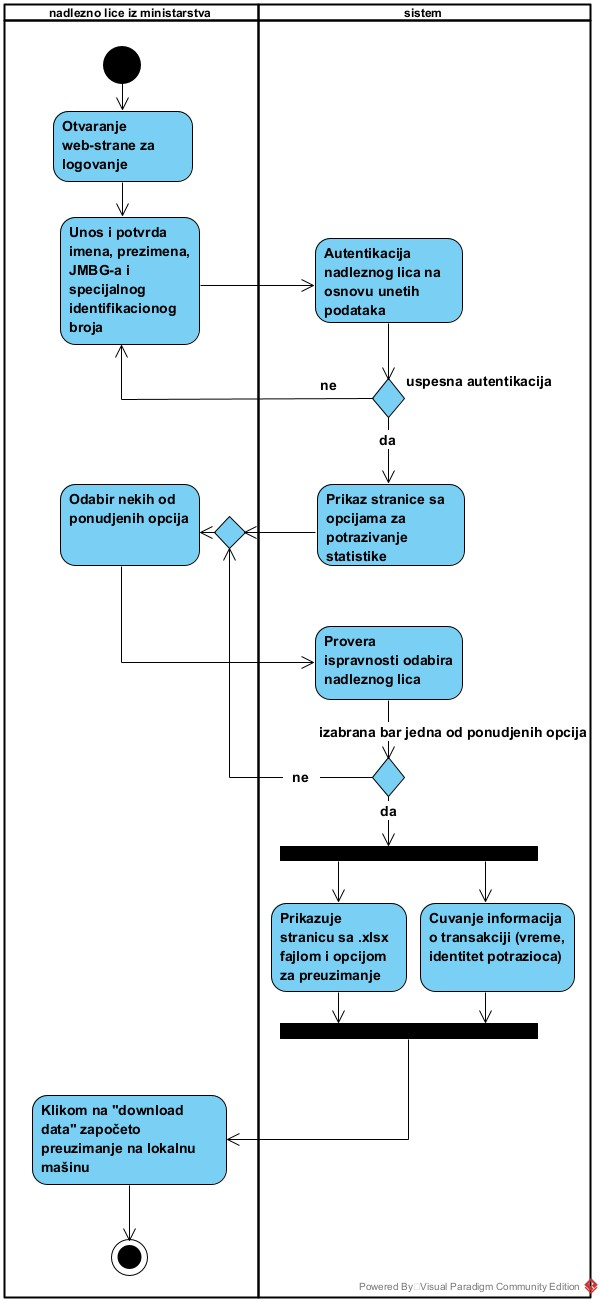
\includegraphics[scale=0.45]{Sprovodjenje_statistike}
\caption{Dijagram aktivnosti - Sprovo\dj{}enje statistike nadle\v{z}nom licu}
\end{figure}

\subsubsection{Slučaj upotrebe: Kol centar}
\begin{itemize}
\item \textbf{Kratak opis:} Osoba poziva kol centar Kovid sistema u cilju informisanja. Dodeljenom opereteru može postavljati pitanja koja se tiču terapije, vakcinacije, simptoma, tegoba (naročito posle vakcinacije). Saopštene informacije se čuvaju u sistemu za potrebe dalje analize i izrade statistike u okviru sistema.
\item \textbf{Učesnici:}
\begin{itemize}
    \item Osoba koja poziva kol centar.
    \item Operater koji se dodeljuje osobi za vreme poziva.
\end{itemize}
 \item \textbf{Preduslovi:} Sistem je aktivan. Osoba poseduje mobilni ili fiksni telefon. Postoje aktivni operateri.
 \item \textbf{Postuslovi:} Osoba je dobila odgovore na sva pitanja koja je postavila operateru. Sistem ažurira podatke o tekućem razgovoru.
 \item \textbf{Osnovni tok:}
 \begin{enumerate}
    \item Osoba poziva broj telefona kol centra.
    \item Sistem preusmerava poziv prvom slobodnom operateru.
    \item Osoba i operater otpočinju razgovor u kom operater odgovara na postavljena pitanja.
    \item Razgovor se završava.
 \end{enumerate}
 \item \textbf{Alternativni tokovi:}
 \begin{itemize}
            \item[A1.] \textbf{Prekid veze} Ukoliko nakon koraka 2 osnovnog toka sistema dođe do tehničkih smetnji ili obustave poziva, razgovor biva prekinut.
        \end{itemize}
 \item \textbf{Dodatne informacije:}
            \begin{itemize}
                \item Kol centar poseduje jedinstveni servisni broj otvoren od strane regulatornog tela.
                \item Svi pozivaoci bivaju preusmereni na određeni lokal, dok se operater dodeljuje prema listi čekanja.
            \end{itemize}

\end{itemize}

\begin{figure}[H]
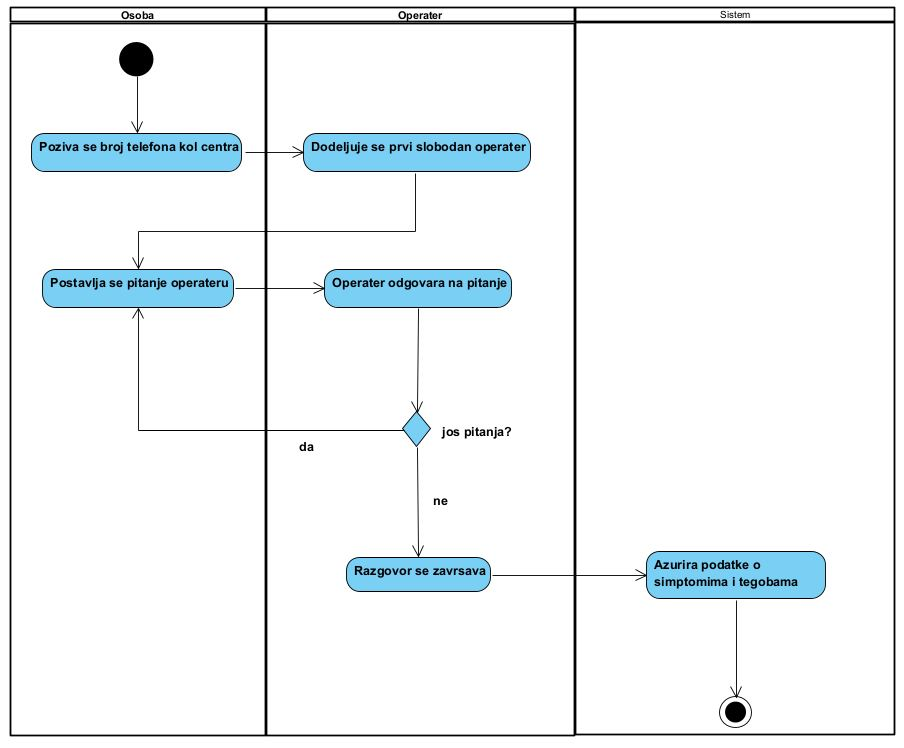
\includegraphics[width=\textwidth,height=\textheight,keepaspectratio]{Kol_centar}
\caption{Dijagram aktivnosti - Kol centar}
\end{figure}

\subsection{Kovid propusnice}

U ovom poglavlju se bavimo formalizacijom rada sa kovid propusnicama. U nastavku su opisani slučajevi upotrebe izdavanja i validacije kovid propusnica. Na Slici \ref{slk:propusnica} prikazan je niz stanja u kojima se može naći kovid propusnica.

\begin{figure}[H]
\centering
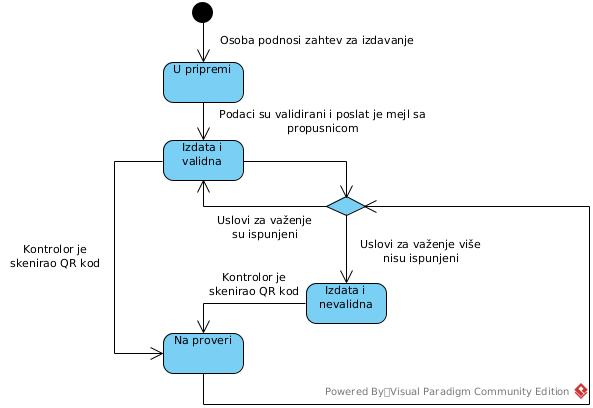
\includegraphics[scale=0.6]{Kovid_propusnica}
\caption{Dijagram stanja - Kovid propusnica}
\label{slk:propusnica}
\end{figure}

\subsubsection{Slučaj upotrebe: Izdavanje kovid propusnice}

%Prvih 5 tacaka je obavezno, ostale nisu - navesti potrebne
%Ne bi bilo loše da, ako se dodaje neki dijagram, stoji opis uz njega i da se negde u tekstu onda reveriše na tu sliku

\begin{itemize}
    \item \textbf{Kratak opis:} Registrovana osoba bira opciju za podnošenje zahteva za kovid propusnicu. Sistem proverava podatke, izdaje propusnicu i vraća odgovarajuću poruku.
    \item \textbf{Učesnici:}
        \begin{itemize}
            \item Registrovana osoba - želi brzo da dobije kovid propusnicu uz minimalan broj koraka
        \end{itemize}
    \item \textbf{Preduslovi:} Sistem je aktivan. Osoba je registrovana i ima pristup internetu.
    \item \textbf{Postuslovi:} Sistem je izdao propusnicu registrovanoj osobi.
    \item \textbf{Osnovni tok:}
        \begin{enumerate}
            \item Osoba otvara stranicu za prijavu.
            \item Sistem prikazuje formular za prijavu.
            \item Osoba unosi odgovarajuće podatke.
            \item Osoba potvrđuje unos.
            \item Sistem vrši validaciju podataka.
            \item Osoba otvara stranicu za podnošenje zahteva za izdavanje propusnice.
            \item Sistem prikazuje tri moguće opcije:
                \begin{itemize}
                    \item Izdavanje propusnice na osnovu primljene vakcine.
                    \item Izdavanje propusnice na osnovu negativnog PCR ili antigenskog testa.
                    \item Izdavanje propusnice na osnovu preležanog virusa.
                \end{itemize}
            \item Osoba bira jednu od ponuđenih opcija.
            \item Sistem proverava zadovoljenost uslova.
            \item Sistem osobi šalje mejl sa kovid propusnicom.
            \item Sistem obaveštava osobu da je operaciju uspešno izvršena i da je propusnica poslata.
        \end{enumerate}
     
    %Ako postoje, podtokove nazivati sa P1, P2, ...   
    %\item \textbf{Podtokovi:}    
    
    %Alternativne tokove nazivati sa A1, A2, ...
    \item \textbf{Alternativni tokovi:}
        \begin{itemize}
            \item[A1.] \textbf{Neuspešno prijavljivanje.} Ukoliko u koraku 5 osnovnog toka sistem naiđe na neispravne podatke, obaveštava osobu i zahteva ponovni unos podataka. Proces se nastavlja u koraku 3 osnovnog toka.
            \item[A2.] \textbf{Uslovi za izdavanje nisu zadovoljeni.} Ukoliko u koraku 9 osnovnog toga sistem ustanovi da nisu zadovoljeni odgovarajući uslovi za izdavanje propusnice, obaveštava osobu. Proces se završava.
        \end{itemize}
    
    %Ako postoje, specijalne zahteve navesti ovde
    %\item \textbf{Specijalni zahtevi:}
        
    \item \textbf{Dodatne informacije:}
        \begin{itemize}
            \item Podaci koji su potrebni za prijavu na sistem su korisničko ime i lozinka.
            \item Uslovi za izdavanje propusnice su:
                \begin{itemize}
                    \item Druga doza vakcine je primljena pre manje od 7 meseci ili  je primljena treća doza vakcine.
                    \item Postojanje negativnog PCR testa koji nije stariji od 72 sata ili antigenskog testa koji nije stariji od 48 sati.
                    \item Virus je preležan pre manje od 7 meseci.
                \end{itemize}
            \item Kovid propusnica sadrži QR kod na osnovu kog se proverava validnost propusnice.
        \end{itemize}
\end{itemize}

\begin{figure}[H]
\centering
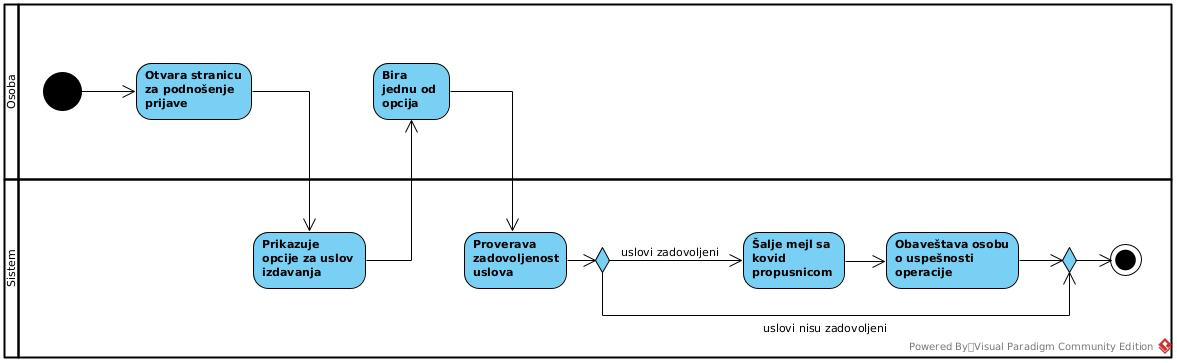
\includegraphics[scale=0.25]{Izdavanje_propusnice}
\caption{Dijagram aktivnosti - Izdavanje kovid propusnice}
\label{slk:izdavanje}
\end{figure}

\subsubsection{Slučaj upotrebe: Validacija kovid propusnica}

\begin{itemize}
    \item \textbf{Kratak opis:} Kontrolor očitava QR kod sa kovid propusnice. Sistem proverava podatke i prikazuje odgovarajuću poruku o validnosti propusnice.
    \item \textbf{Učesnici:}
        \begin{itemize}
            \item Kontrolor - želi brzo da proveri validnost kovid propusnice
        \end{itemize}
    \item \textbf{Preduslovi:} Sistem je aktivan. Kontrolor ima pristup internetu.
    \item \textbf{Postuslovi:} Sistem je obavestio kontrolora o validnosti kovid propusnice.
    \item \textbf{Osnovni tok:}
        \begin{enumerate}
            \item Kontrolor očitava QR kod sa kovid propusnice.
            \item Kontrolor otvara stranicu za validaciju.
            \item Sistem dobija zahtev za validaciju propusnice.
            \item Sistem proverava zadovoljenost uslova za važenje propusnice.
            \item Sistem prikazuje podatke o vlasniku propusnice i status propusnice:
                \begin{itemize}
                    \item Zeleno - ukoliko su uslovi za važenje propusnice zadovoljeni.
                    \item Crveno - ukoliko uslovi za važenje propusnice nisu zadovoljeni.
                \end{itemize}
        \end{enumerate}
    \item \textbf{Specijalni zahtevi:}
        \begin{itemize}
            \item Kontrolor poseduje uređaj kojim se može skenirati QR kod.
        \end{itemize}
    \item \textbf{Dodatne informacije:}
        \begin{itemize}
            \item Uslovi za važenje propusnice su:
                \begin{itemize}
                    \item Druga doza vakcine je primljena pre manje od 7 meseci ili  je primljena treća doza vakcine.
                    \item Postojanje negativnog PCR testa koji nije stariji od 72 sata ili antigenskog testa koji nije stariji od 48 sati.
                    \item Virus je preležan pre manje od 7 meseci.
                \end{itemize}
        \end{itemize}
\end{itemize}

\begin{figure}[H]
\centering
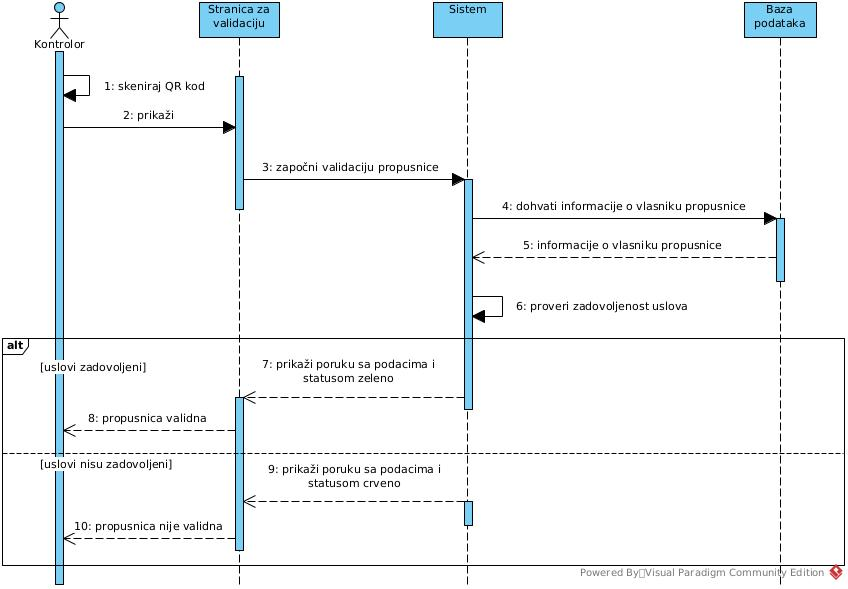
\includegraphics[scale=0.5]{Validacija_propusnice}
\caption{Dijagram sekvence - Validacija kovid propusnice}
\label{slk:validacija}
\end{figure}

\subsection{Testiranje}

U ovom poglavlju se bavimo formalizacijom procesa testiranja registrovanih osoba.

\subsubsection{Slučaj upotrebe: Testiranje osobe PCR ili Antigen testom}

\begin{itemize}
    \item \textbf{Kratak opis:} Osoba odlazi u kovid ambulantu kako bi se testirala PCR ili antigenskim testom. Nakon identifikacije, osoba popunjava formular i ide na testiranje. Medicinski radnik koji vrši testiranje čeka rezultate i osobi šalje mejl sa podacima o ishodu testa, ažurirajući pritom bazu podataka radi dobijanja kovid propusnica i sl.
    \item \textbf{Učesnici:}
        \begin{itemize}
            \item Osoba
            \item Medicinski radnik - osoblje zaposleno u ambulanti
        \end{itemize}
    \item \textbf{Preduslovi:} Sistem je aktivan. Osoba ima pristup internetu.
    \item \textbf{Postuslovi:} Osoba dobija mejl sa rezultatom testa. Sistem je ažuriran.
    \item \textbf{Osnovni tok:}
        \begin{enumerate}
           \item Osoba ulazi u ambulantu.
           \item Radnik traži lični dokument na uvid i daje osobi formular koji treba popuniti. \item Osoba u formularu bira jedan od dva testa:
           \begin{itemize}
               \item PCR test
               \item Sars-Cov-2 Antigen test
           \end{itemize}
           \item Osoba potpisuje formular.
           \item Radnik upisuje podatke o osobi sa formulara.
           \item Osoba ide na testiranje.
           \item Radnik čeka rezultate. Nakon čekanja rezultata, radnik šalje osobi rezultate testa na mejl sa formulara.
           \item Radnik ažurira bazu podataka. Sistem je ažuriran.
        \end{enumerate}
    \item \textbf{Specijalni zahtevi:}
        \begin{itemize}
            \item Osoba kod sebe mora imati važeći lični dokument.
        \end{itemize}
    \item \textbf{Dodatne informacije:}
        \begin{itemize}
            \item Osoba u formularu upisuje:
            \begin{itemize}
                \item Ime
                \item Prezime
                \item JMBG
                \item E-mail adresu
            \end{itemize}
            \item Ukoliko je rezultat PCR testa pozitivan, osoba ima virus i mora ostati u kućnoj izolaciji naredne 2 nedelje. Ukoliko je rezultat negativan, osoba dobija pravo na kovid propusnicu.
            \item Ukoliko je rezultat Sars-Cov-2 Antigen testa pozitivan, osoba dobija pravo na kovid propusnicu prema važećim uslovima. Ukoliko je rezultat negativan, osoba treba preduzeti sve mere predostrožnosti kako bi se zaštitila od infekcije.
            \item Ukoliko je rezultat bilo kog testa nevalidan, osoba snosi troškove testiranja i poziva se na ponovno testiranje.
        \end{itemize}
\end{itemize}

\begin{figure}[H]
\centering
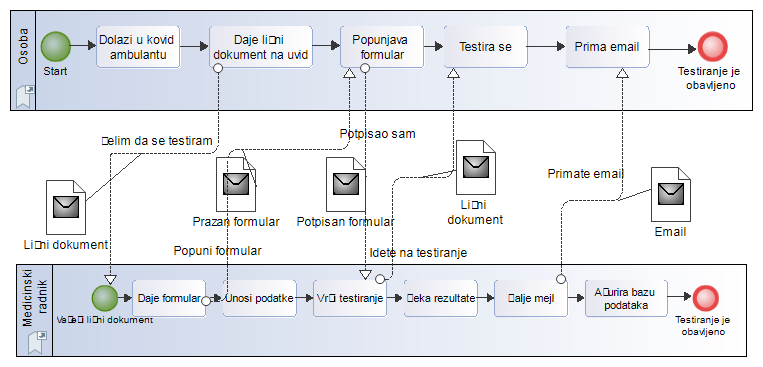
\includegraphics[scale=0.5]{Dijagram_testiranje}
\caption{BPMN dijagram saradnje - testiranje}
\end{figure}

\subsection{Kućna izolacija}
U ovom poglavlju bavimo se implementacijom procesa kućne izolacije, počev od evidentiranja, preko praćenja izolacije, do prestanka izolacije.
\subsubsection{Slučaj upotrebe: Evidentiranje zaražene osobe}
\begin{itemize}
    \item \textbf{Kratak opis:} Medicinski radnik na osnovu pozitivnog PCR testa šalje osobi instrukcije o izolaciji i ažurira informacioni sistem kako bi se zaražene osobe mogle pratiti u narednom periodu.
    \item \textbf{Učesnici:}
        \begin{itemize}
            \item Medicinski radnik
        \end{itemize}
    \item \textbf{Preduslovi:} Sistem je aktivan. Medicinski radnik ima dozvolu za menjanje podataka o zaraženim licima.
    \item \textbf{Postuslovi:} Sistem obaveštava radnika o uspešnosti izmena.
    \item \textbf{Osnovni tok:}
    \begin{enumerate}
        \item Medicinski radnik otvara stranicu za logovanje i unosi svoje podatke.
        \item Sistem dozvoljava radniku da dođe do podataka o zaraženim licima.
        \item Medicinski radnik unosi podatke o zaraženom i dužinu trajanja izolacije.
        \item Medicinski radnik potvrđuje unos.
        \item Sistem prikazuje povratnu informaciju medicinskom radniku.
        \item Sistem obaveštava osobu da je u obavezi da primeni kućnu izolaciju.
    \end{enumerate}
    \item\textbf{Alternativni tokovi:}
        \begin{itemize}
            \item [A1.] \textbf{Neuspešan unos podataka.} Ukoliko u koraku 5 glavnog toka sistem obavesti radnika da podaci o zaraženom nisu validni, baza podataka o zaraženima ostaje neizmenjena i proces se završava.
        \end{itemize}
\end{itemize}
\subsubsection{Slučaj upotrebe: Provera poštovanja izolacije}
\begin{itemize}
    \item \textbf{Kratak opis:} Osoba se poziva iz kol centra kako bi se ispratilo njeno poštovanje mera kućne izolacije.
    \item \textbf{Učesnici:}
        \begin{itemize}
            \item Zaražena osoba
            \item Operater
        \end{itemize}
    \item \textbf{Preduslovi:} Sistem je aktivan. Osoba poseduje mobilni ili fiksni telefon.
    \item \textbf{Postuslovi:} Operater dobija tačne informacije o ponašanju osobe koja treba da je u izolaciji.
    \item \textbf{Osnovni tok:}
        \begin{enumerate}
            \item Operater otvara stranicu za logovanje.
            \item Operater unosi svoje podatke i potvrđuje unos.
            \item Sistem odobrava pristup.
            \item Operater zahteva podatke o zaraženima.
            \item Sistem prikazuje tabelu sa zaraženim osobama.
            \item Operater nasumično bira broj telefona osobe koja treba da bude u kućnoj izolaciji.
            \item Operater razgovara sa osobom i zaključuje o poštovanju kućne izolacije.
        \end{enumerate}
    \item\textbf{Alternativni tokovi:}
        \begin{itemize}
            \item[A1.] \textbf{Operater nema dozvolu za pristup.} Ukoliko u koraku 3 sistem ne odobri pristup, proces se završava.
        \end{itemize}
    \item \textbf{Dodatne informacije:}
        \begin{itemize}
            \item Ukoliko operater sumnja na nepoštovanje mera kućne izolacije, o tome obaveštava organe reda kako bi se utvrdilo tačno stanje zaraženog i preduzele odgovarajuće mere.
            \item Ukoliko se osoba požali na tegobe, operater je dužan da obavesti medicinsku službu kako bi se pravovremeno reagovalo.
        \end{itemize}
\end{itemize}
\subsubsection{Slučaj upotrebe: Produžavanje izolacije}
\begin{itemize}
    \item \textbf{Kratak opis:} Nakon isteka predviđenih mera kućne izolacije, osoba se poziva na ponovno testiranje kako bi se utvrdilo da li izolaciju treba nastaviti.
    \item \textbf{Učesnici:}
        \begin{itemize}
            \item Operater
        \end{itemize}
    \item \textbf{Preduslovi:} Sistem je aktivan. Operater je autorizovan za pristup podacima o zaraženima.
    \item \textbf{Postuslovi:} Operater je obavestio osobu o ponovnom testiranju.
    \item \textbf{Osnovni tok:}
        \begin{enumerate}
            \item Operater otvara stranicu za logovanje.
            \item Operater unosi svoje podatke i potvrđuje unos.
            \item Sistem odobrava pristup.
            \item Operater zahteva podatke o zaraženima.
            \item Sistem prikazuje tražene podatke.
            \item Operater bira osobu kojoj je tog dana istekla kućna izolacija.
            \item Operater pronalazi podatke o osobi i pozivom je obaveštava da je potrebno ponovno testiranje.
        \end{enumerate}
\end{itemize}

\subsection{Dobavljanje medicinskih sredstava}

\subsubsection{Slučaj upotrebe: Dodela specijalnog identifikacionog broja za u\v{c}estvovanje u transakciji zaliha}
\begin{itemize}
    
\item \textbf{Kratak opis:} Ministarstvo zdravlja sistemu dostavlja podatke  o licima koja \'{c}e biti nadle\v{z}na za regulisanje transakcije  novih zaliha vakcina i testova. Nakon provere podataka, sistem za svako od odabranih lica vr\v{s}i registraciju na sistem i generi\v{s}e specijalni identifikacioni broj koji će se koristiti pri logovanju za odgovaranje na zahtev za dostavljanje zaliha vakcina i testova i pri logovanju za potvrdu uspe\v{s}no izvr\v{s}ene transakcije zaliha. 
\item \textbf{Učesnici:}
\begin{itemize}
    \item Nadležno lice ministarstva zdravlja
\end{itemize}
 \item \textbf{Preduslovi:} Sistem je aktivan. Učesnik ima pristup internetu.
 \item \textbf{Postuslovi:} Sva lica iz ministarstva nadle\v{z}na za odgovaranje na zahtev za dostavljanje novih zaliha poseduje poseban identifikacioni broj koji će koristiti pri logovanju na sistem u svrhu odgovaranja na zahtev za nove zalihe.
 \item \textbf{Osnovni tok:}
 \begin{enumerate}
    \item Lice iz ministarstva zdravlja formira spisak nadle\v{z}nih lica za odgovoranje na zahtev kovid ambulanti za dostavljanje novih zaliha.
    \item Lice iz ministarstva taj spisak putem sigurnih kanala elektronskom poštom biva dostavljen do informacionog sistema.
    \item Koristeći u pozadini posebne he\v{s} funkcije , sistem generi\v{s}e identifikacione brojeve.
    \item Sistem, svaki od identifikacionih brojeva putem sigurnih kanala elektronskom poštom dostavlja svakom od lica iz ministarstva koje se na\v{s}lo na spisku nadle\v{z}nih za odgovoranje na zahtev kovid ambulanti za dostavljanje novih zaliha.
    \item Svako od nadle\v{z}nih lica za odgovaranje na zahtev za dostavljanje zaliha sistem registruje, i obaveštava da \'{c}e za logovanje na sistem za potrebe odgovora na zahtev za dostavljanje zaliha koristiti dodeljen identifikacioni broj.
 \end{enumerate}
\end{itemize}

\begin{figure}[H]
\centering
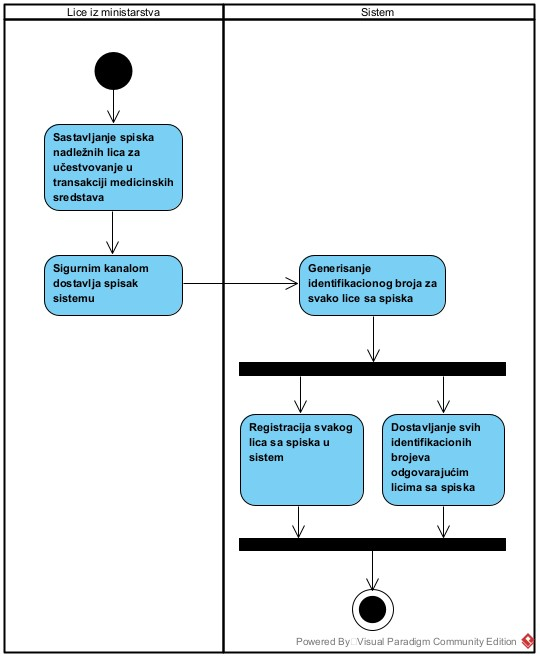
\includegraphics[scale=0.5]{DodelaIDZaTransakcijuZaliha}
\caption{Dijagram aktivnosti -  Dodela specijalnog identifikacionog broja za u\v{c}estvovanje u transakciji zaliha}
\end{figure}

\subsubsection{Slučaj upotrebe: Potra\v{z}ivanje novih zaliha vakcina i testova}
\begin{itemize}
\item \textbf{Kratak opis:} Nakon \v{s}to neka od kovid ambulanti ostane sa nezadovoljavaju\'{c}om koli\v{c}inom vakcina i/ili testova nekog od proizvo\dj{}a\v{c}a,  nakon neophodnih provera, sistem kroz nekoliko koraka nudi mogu\'{c}nost slanja zahteva ministarstvu zdravlja kojim se potra\v{z}uju neophodne zalihe vakcina i/ili testova, a nadle\v{z}no lice iz ministarstva \v{s}alje povratnu informaciju o mogu\v{c}nostima ispunjenja podnetog zahteva.
\item \textbf{Učesnici:}
\begin{itemize}
    \item \v{C}lan medicinskog osoblja kovid ambulante.
    \item  Nadle\v{z}no lice iz ministarstva zdravlja.
\end{itemize}
 \item \textbf{Preduslovi:} Sistem je aktivan. Svi u\v{c}esnici imaju pristup internetu.
 \item \textbf{Postuslovi:} Ministarstvo zdravlja je prihvatilo zahtev i poslalo povratnu informaciju o mogu\'{c}nostima ispunjenja zahteva kovid ambulante.
 \item \textbf{Osnovni tok:}
 \begin{enumerate}
    \item \v{C}lan medicinskog osoblja otvara stranicu za podno\v{s}enje zahteva.
    \item Sistem mu prikazuje stranicu sa formularom.
    \item \v{C}lan medicinskog osoblja popunjava formular koji je neophodan za autentikaciju. Formular sadr\v{z}i polje za ime, prezime, JMBG, informacije o kovid ambulanti iz koje se zahtev \v{s}alje.
    \item \v{C}lan medicinskog osoblja potvr\dj{}uje unos.
    \item Sistem vr\v{s}i validaciju unetih podataka.
    \item Sistem \v{c}lanu medicinskog osoblja prikazuje stranicu sa formularom za podno\v{s}enje zahteva koji je formatiran tako da se pored svakog od proizvo\dj{}a\v{c}a nalazi polje za unos broja zahtevanih vakcina  odgovaraju\'{c}eg proizvo\dj{}a\v{c}a i polje za unos broja zahtevanih testova.  
    \item \v{C}lan medicinskog osoblja popunjava formular i potvr\dj{}uje unos.
    \item Sistem proverava ispravnost popunjenog formulara.
    \item Sistem podnetom zahtevu dodeljuje identifikacioni broj. 
    \item Sistem zahtev prosle\dj{}uje nekom od lica iz ministarstva zadu\v{z}enom za slanje povratne informacije o mogu\v{c}nostima ispunjenja zahteva.
    \item Nadle\v{z}no lice ministarstva otvara stranicu za logovanje
    \item Sistem nadle\v{z}nom licu prikazuje stranicu i zahteva da se popune polja za ime, prezime, JMBG i poseban identifikacioni broj specijalno dodeljen za ovaj vid transakcija.
    \item Nadle\v{z}no lice ministarstva unosi podatke i potvr\dj{}uje unos.
    \item Sistem proverava validnost unetih podataka.
    \item Nadle\v{z}no lice iz ministarstva odgovara na zahtev.
    \item Kao propratna informacija \v{c}lanu medicinskog osoblja salje se vremenski interval (du\v{z}ine najvi\v{s}e 8 sati) u okviru kojeg se o\v{c}ekuje da transport zatra\v{z}enih zaliha bude realizovan.
    \item Identifikacioni broj zahteva, informacije o vremenu, zatra\v{z}enim zalihama, povratnoj informaciji, identitetu podnosioca zahteva kao i o  identitetu lica iz ministarstva zdravlja koje je na zahtev odgovorilo \v{c}uvaju se u sistemu.
 \end{enumerate}
 \item \textbf{Alternativni tokovi:}
 \begin{itemize}
            \item[A1.] \textbf{Neuspe\v{s}na dodela dozvole za podno\v{s}eje zahteva.} Ukoliko u koraku 5 osnovnog toka sistem naiđe na neispravne podatke, obaveštava korisnika i zahteva ponovni unos podataka. Proces se nastavlja u koraku 3 osnovnog toka.
            \item[A2.] \textbf{Neispravno podno\v{s}enje zahteva.} Ukoliko u koraku 8 osnovnog toka sistem utvrdi da \v{c}lan medicinskog osoblja nije popunilo formular kako je predvi\dj{}eno, on o tome biva obave\v{s}teno. Proces se nastavlja u koraku 6 osnovnog toka. 
            \item[A3.] \textbf{Neuspe\v{s}na dodela dozvole za odgovor na zahtev.} Ukoliko u koraku 14. sistem utvrdi gre\v{s}ku pri autentikaciji, o tome obave\v{s}tava u\v{c}esnika. Proces se nastavlja u koraku 12. 
            \item[A4.] \textbf{Odbijen zahtev za dostavljanje zaliha} Ukoliko je u koraku 15. nadle\v{z}no lice iz ministarstva uputilo negativan odgovor, kao propratnu informaciju \v{c}lanu medicinskog osoblja pored obrazlo\v{z}enja odluke, \v{s}alje na koju kovid ambulatni je eventualno potrebno preusmeriti pacijente (na osnovu lokacije i preostalih zaliha). Proces se nastavlja u koraku 17 osnovnog toka.
        \end{itemize}
\end{itemize}

\begin{figure}[H]
\centering
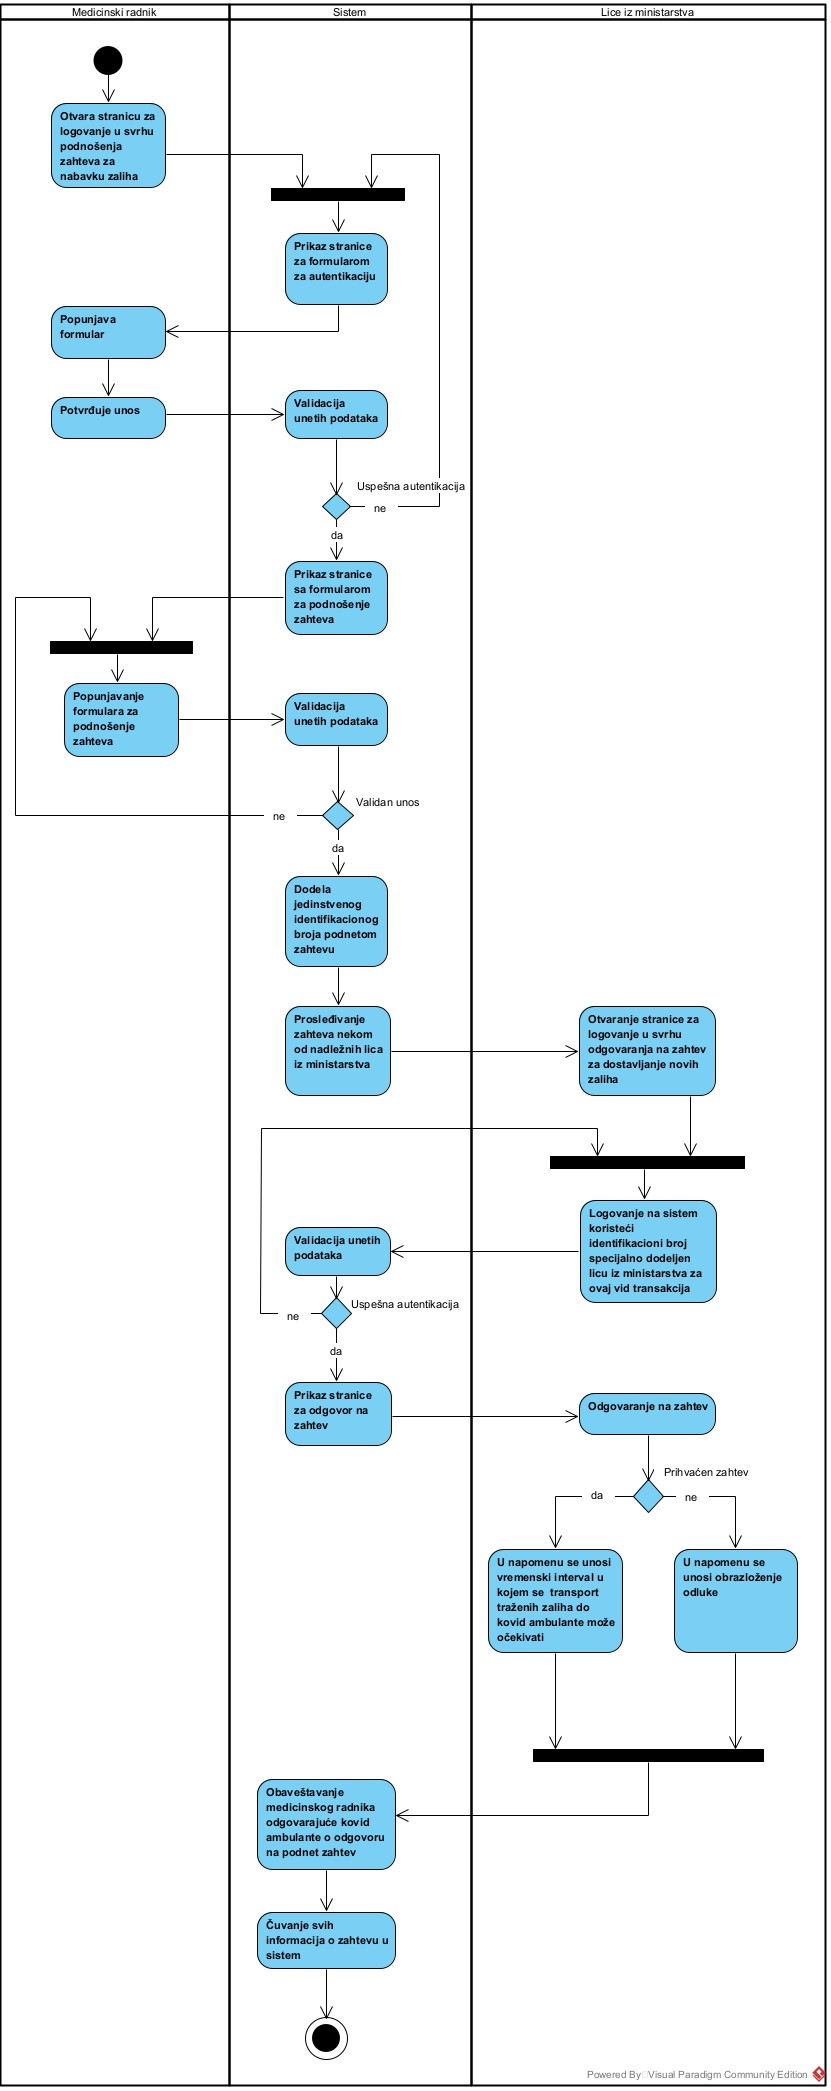
\includegraphics[scale=0.3]{Potrazivanje_novih_zaliha}
\caption{Dijagram aktivnosti -  Potraživanje novih zaliha}
\end{figure}

\subsubsection{Slučaj upotrebe: Prijem novih zaliha}
\begin{itemize}
\item \textbf{Kratak opis:} Nakon \v{s}to se kovid ambulanti na raspolaganje stavi nova koli\v{c}ina zaliha, de\v{z}urni \v{c}lan medicinskog osoblja \v{s}alje povratnu informaciju o uskla\dj{}enosti potra\v{z}enih i pristiglih zaliha.
\item \textbf{Učesnici:}
\begin{itemize}
    \item \v{C}lan medicinskog osoblja kovid ambulante
    \item Nadle\v{z}no lice iz ministarstva zdravlja
    \item Profesionalni vozač angažovan od strane ministarstva zdravlja
\end{itemize}
 \item \textbf{Preduslovi:} Sistem je aktivan.Član medicinskog osoblja i nadležno lice iz ministarstva zdravlja imaju pristup internetu.
 \item \textbf{Postuslovi:} Kovid ambulanti su dostavljene potra\v{z}ene zalihe i podaci u sistemu su a\v{z}urirani 
 \item \textbf{Osnovni tok:}
 \begin{enumerate}
    \item Ministarstvo zdravlja upu\'{c}uje transportno vozilo sa zahtevanim zalihama i vozaču predaje fizički formular  sa identifikacionim brojem zahteva na osnovu kojeg se zalihe dostavljjaju i praznim poljem za potpis primaoca i napomenu.
   \item  Vozač prevozi robu.
    \item Voza\v{c} \v{c}lanu medicinskog osoblja daje fizi\v{c}ki formular.
    \item \v{C}lan medicinskog osoblja daje svoj potpis voza\v{c}u.
    \item \v{C}lan medicinskog osoblja otvara stranicu za prihvatanje novih zaliha.
    \item Sistem prikazuje stranicu sa formularom koji sadr\v{z}i polje za ime, prezime, jmbg i identifikacioni broj zahteva za potra\v{z}ivanje zaliha.
    \item \v{C}lan medicinskog osoblja unosi li\v{c}ne podatke i identifikacioni broj zahteva koji se nalazi u formularu koji je dobio od voza\v{c}a.
    \item \v{C}lan medicinskog osoblja potvr\dj{}uje unos.
    \item Sistem vr\v{s}i validaciju unetih podataka.
    \item Sistem \v{c}lanu medicinskog osoblja prikazuje stranicu sa informacijama o podnetom zahtevu ( informacije o vremenu podnetog zahteva, zatra\v{z}enim zalihama, povratnoj informaciji, identitetu podnosioca zahteva )
    \item Medicinski radnik utvr\dj{}uje da li se koli\v{c}ina pristiglih zaliha poklapa sa onom koja je zahtevana.
    \item \v{C}lan medicinskog osoblja vr\v{s}i prenos robe u skladi\v{s}te.
    \item Voza\v{c} potpisanu  potvrdu o primljenim zalihama daje nadle\v{z}nom licu za regulisanje zaliha.
    \item Nadle\v{z}no lice otvara stranicu logovanje u svrhu potvrde uspe\v{s}ne transakcije zaliha.
    \item Sistem mu prikazuje stranicu sa formularom sa poljima za ime, prezime, jmbg i specijalni identifikacioni broj.
    \item Nadle\v{z}no lice ministarstva unosi podatke i potvr\dj{}uje unos.
    \item Sistem proverava validnost unetih podataka.
    \item Nadle\v{z}no lice unosi informacije o transakciji zaliha (identifikacioni broj zahteva, identitet de\v{z}urnog \v{c}lana medicinskog osoblja koje je potvrdilo dostavu zatra\v{z}enih zaliha).
    \item Sistem sve informacije o transakciji \v{c}uva i a\v{z}urira podatke vezane za preostale zalihe u odgovaraju\'{c}oj kovid ambulanti.
 \end{enumerate}
 \item \textbf{Alternativni tokovi:}
 \begin{itemize}
            \item[A1.] \textbf{Neuspe\v{s}na dodela dozvole za proveru uskla\dj{}enosti potra\v{z}enih i pristiglih zaliha.} Ukoliko u koraku 9 osnovnog toka sistem naiđe na neispravne podatke, obaveštava korisnika i zahteva ponovni unos podataka. Proces se nastavlja u koraku 5 osnovnog toka.
	\item [A2.] \textbf{Nepoklapanje u broju zahtevanih i pristiglih zaliha.} Ukoliko je u koraku 11. uo\v{c}eno nepoklapanje pristiglih zaliha sa onom koja je zahtevana, medicinski radnik u formularu koji je potpisao u koraku broj 4. osnovnog roka upisuje napomenu o nepoklapanju. Voza\v{c} popunjen formular dostavlja nadle\v{z}nom licu iz ministarstva, proces se tu zavr\v{s}ava i neophodno je ponoviti transport.
            \item[A3.] \textbf{Neuspe\v{s}na dodela dozvole za potvrdu uspe\v{s}ne transkacije.} Ukoliko u koraku 17. sistem utvrdi gre\v{s}ku pri autentikaciji, o tome obave\v{s}tava u\v{c}esnika. Proces se nastavlja u koraku 15. 
        \end{itemize}
\end{itemize}

\begin{figure}[H]
\centering
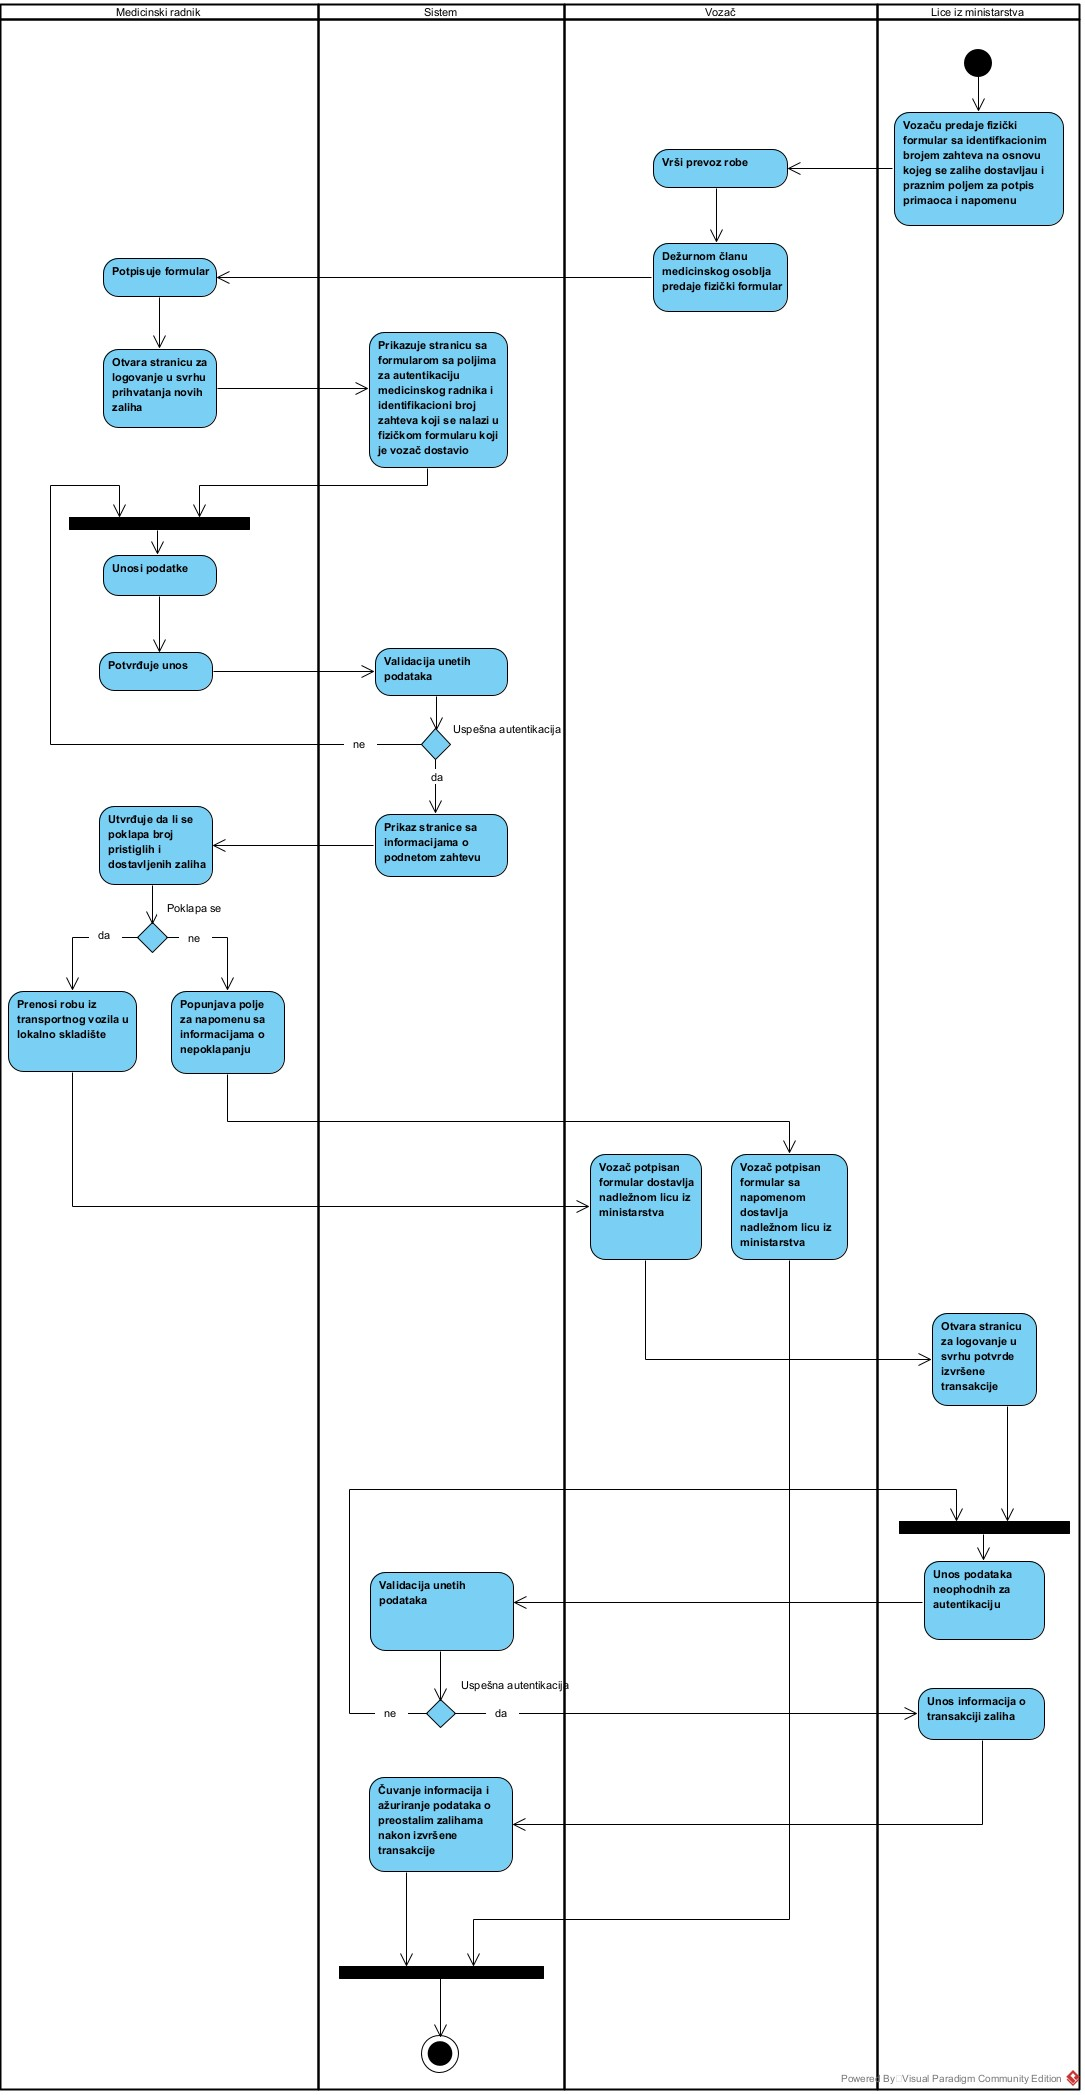
\includegraphics[scale=0.3]{Prijem_novih_zaliha}
\caption{Dijagram aktivnosti -  Prijem novih zaliha}
\end{figure}


\subsection{Administracija}

U ovom poglavlju se bavimo administracijom sistema. U nastavku su prikazani neki od poslova koje administrator sistema obavlja.

\subsubsection{Slučaj upotrebe: Dodavanje novog korisnika}

\begin{itemize}
    \item \textbf{Kratak opis:} Administrator prima zahtev, validira podatke i registruje novog korisnika.
    \item \textbf{Učesnici:}
        \begin{itemize}
            \item Administrator
        \end{itemize}
    \item \textbf{Preduslovi:} Sistem je aktivan.
    \item \textbf{Postuslovi:} Novi korisnik je registrovan.
    \item \textbf{Osnovni tok:}
        \begin{enumerate}
            \item Administrator dobija zahtev za registrovanje.
            \item Administrator proverava da li je formular validan.
            \item Administrator otvara stranicu za dodavanje novog korisnika.
            \item Administrator popunjava formular.
            \item Administrator potvrđuje unos.
            \item Administrator šalje obaveštenje da je novi korisnik dodat.
        \end{enumerate}  
    
    \item \textbf{Alternativni tokovi:}
        \begin{itemize}
            \item[A1.] \textbf{Formular nije validan.} Ukoliko u koraku 2 osnovnog toka administrator zaključi da formular nije validan, šalje odgovarajuće obaveštenje. Proces se završava.
        \end{itemize}
\end{itemize}

\begin{figure}[H]
\centering
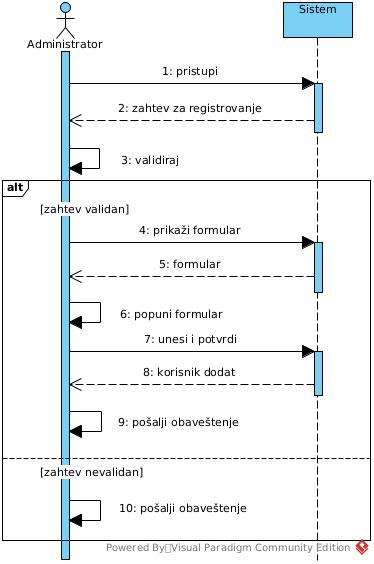
\includegraphics[scale=0.7]{Dodavanje_korisnika}
\caption{Dijagram sekvence - Dodavanje novog korisnika}
\label{slk:dodavanje}
\end{figure}

\subsubsection{Slučaj upotrebe: Pravljenje rezervne kopije baze}

\begin{itemize}
    \item \textbf{Kratak opis:} Administrator pristupa bazi i pravi rezervnu kopiju.
    \item \textbf{Učesnici:}
        \begin{itemize}
            \item Administrator
        \end{itemize}
    \item \textbf{Preduslovi:} Sistem je aktivan.
    \item \textbf{Postuslovi:} Napravljena je rezervna kopija baze.
    \item \textbf{Osnovni tok:}
        \begin{enumerate}
            \item Administrator pristupa bazi sistema.
            \item Administrator proverava da li je u toku neka izmena baze i ako nije prelazi na korak 4.
            \item Administrator čeka da izmena baze bude gotova.
            \item Administrator šalje aktivnim korisnicima sistema da je u toku izrada rezervne kopije baze.
            \item Administrator pravi delimičnu ili kompletnu kopiju baze.
            \item Administrator čuva rezervnu kopiju na odgovarajućoj memorijskoj lokaciji.
            \item Administrator čuva vreme napravljene kopije.
            \item Administrator obaveštava aktivne korisnike sistema da je izrada kopije gotova.
        \end{enumerate}
\end{itemize}

\begin{figure}[H]
\centering
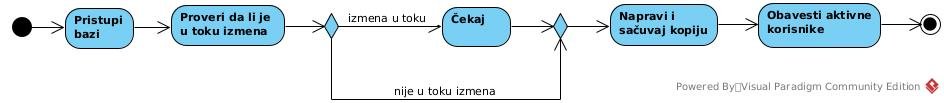
\includegraphics[scale=0.45]{Kopija}
\caption{Dijagram aktivnosti - Pravljenje rezervne kopije baze}
\label{slk:dodavanje}
\end{figure}

\section{Baza podataka}

Na osnovu opisanih slučajeva upotrebe, zaključeno je da je u bazi podataka potrebno čuvati sledeće grupe podataka:

\begin{enumerate}
    \item Osobe (koje se registruju, vakcinišu, testiraju)
    \item Medicinsko osoblje
    \begin{itemize}
        \item Podaci o medicinskim radnicima
        \item Podaci o operaterima
    \end{itemize}
    \item Lica iz ministarstva
    \item Kovid ambulante
    \item Zahtevi
    \begin{itemize}
        \item Podaci o zahtevima za dostavljanje statistike
        \item Podaci o zahtevima za dostavljanje zaliha
    \end{itemize}
    \item Usluge
    \begin{itemize}
        \item Podaci o vakcinaciji
        \item Podaci o testiranju
    \end{itemize}
\end{enumerate}

Na Slici \ref{slk:dijagram_klasa} je prikazan model baze podataka korišćenjem UML dijagrama klasa.
\begin{figure}[H]
	\centering
	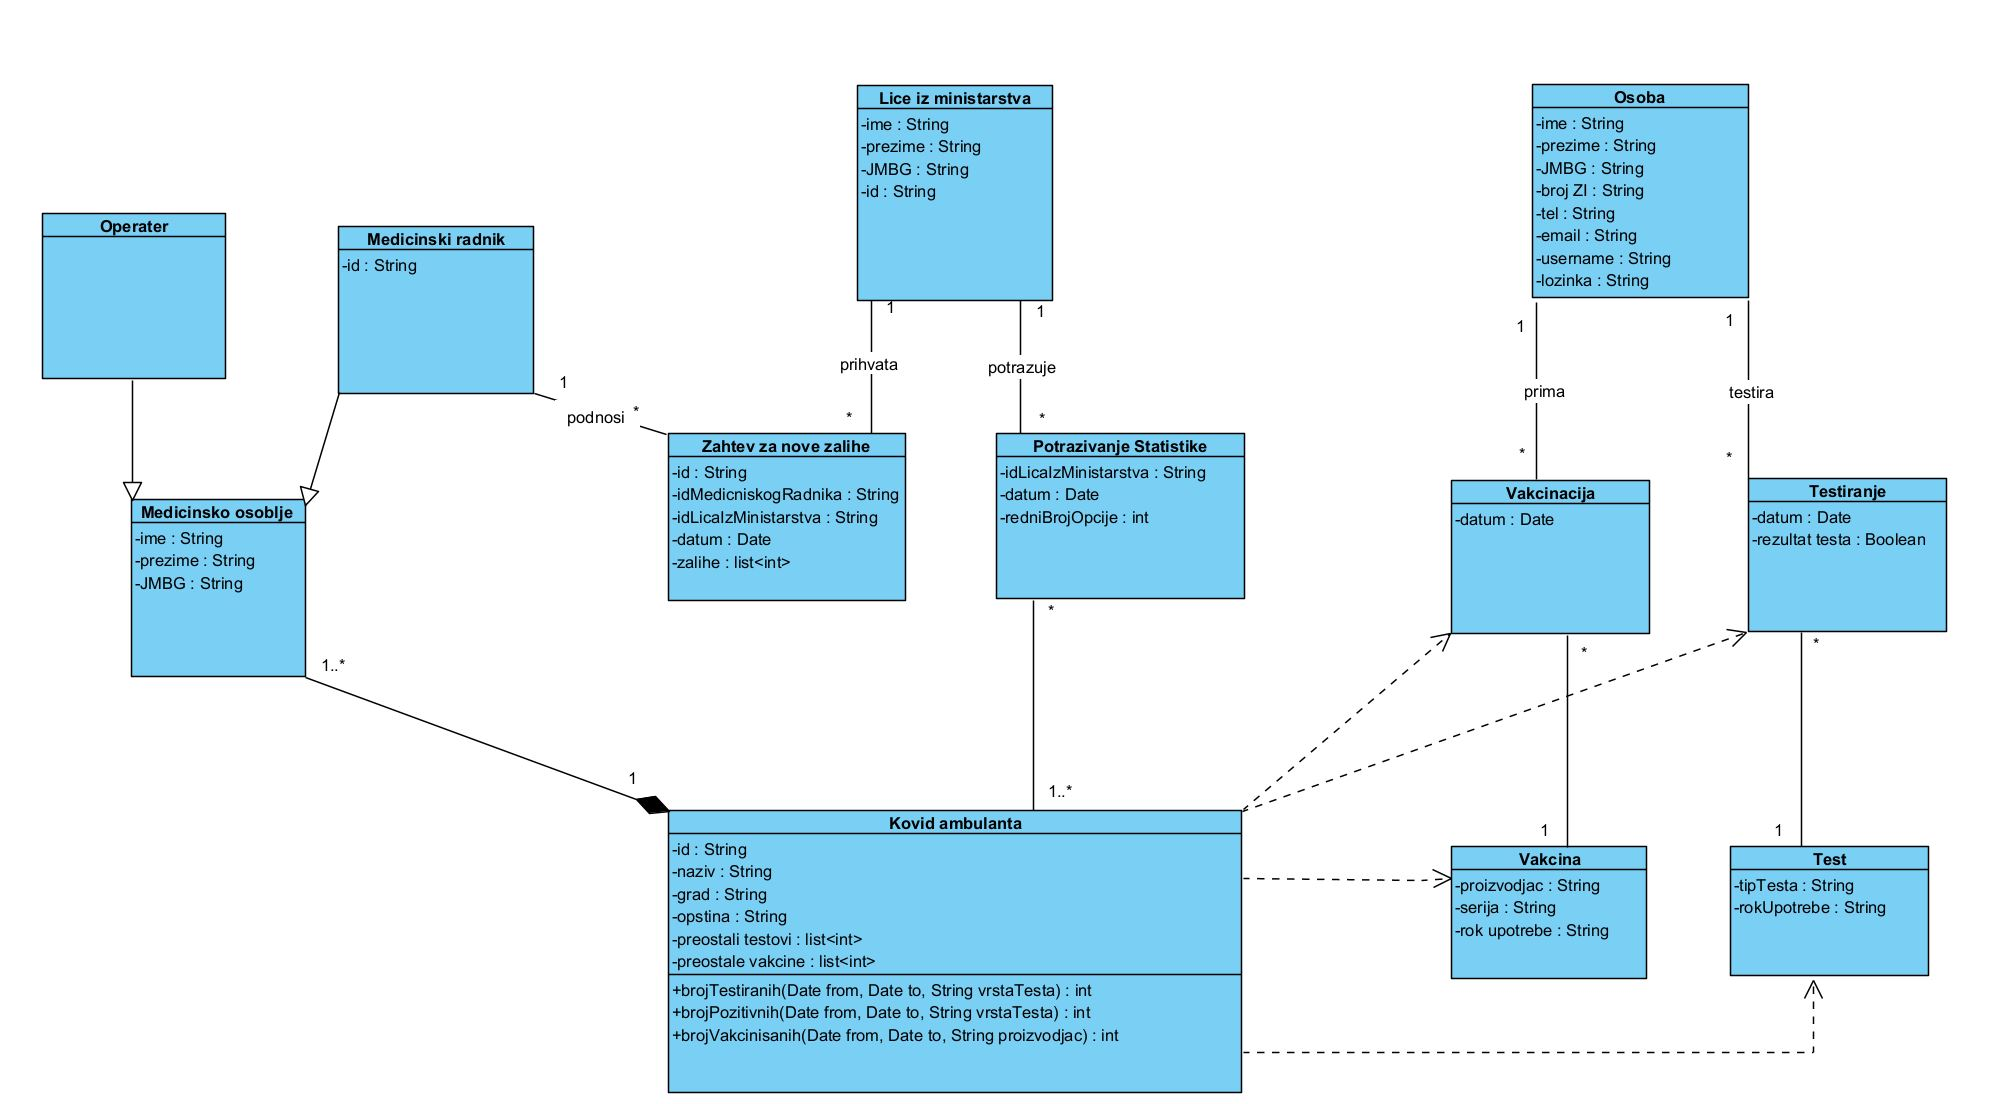
\includegraphics[scale=0.3]{Dijagrami_slike/Dijagram_klasa_podataka.JPG}
	\caption{Dijagram klasa podataka}
	\label{slk:dijagram_klasa}
\end{figure}

\subsection{Podaci o osobama}

Klasa Osoba je jedna od centralnih klasa našeg sistema. Ona predstavlja glavni izvor informacija od značaja za sistem kojima se kroz procese sistema pridružuju dodatne informacije koje se javljaju prilikom odvijanja procesa. \\ \\
Podaci o osobi koji se čuvaju su:

\begin{itemize}
    \item ime
    \item prezime
    \item JMBG
    \item broj ZI (broj zdravstvene knjižice)
    \item telefon
    \item email
    \item username
    \item lozinka
\end{itemize}

Klasa Osoba povezana je sa klasom Vakcinacija vezom "prima" i sa klasom Testiranje vezom "testira".

\subsection{Podaci o medicinskom osoblju}
Klasom Medicinsko osoblje predstavljaju se radnici zdravstvenog sistema i sistema kovid ambulanti.\\ \\
Podaci o medicinskom osoblju:
\begin{itemize}
    \item ime
    \item prezime
    \item JMBG
    \item identifikacioni broj
\end{itemize}
Klasu Medicinsko osoblje nasleđuju klase Medicinski radnik i Operater. Klasa Medicinski radnik predstavlja zaposlene koji pružaju usluge vakcinacije i testiranja. 
Podaci o medicinskom radniku:
\begin{itemize}
    \item id zaposlenog
\end{itemize}
Klasa Operater predstavlja zaposlenog u Kol centru.

\subsection{Podaci o licima iz ministarstva}

Klasa Lice iz ministarstva je klasa podataka koja \v{c}uva podatke o licu iz ministarstva koje u saradnji sa na\v{s}im sistemom mo\v{z}e potra\v{z}ivati statistike kao i odgovarati na pristigle zahteve iz kovid ambulanti vezane za dostavljanje novih zaliha.
\\~\\
Podaci o licu iz ministarstva koji se \v{c}uvaju:
\begin{itemize}
    \item ime
    \item prezime
    \item JMBG
    \item identifikacioni broj
\end{itemize}

Klasa Lice iz ministarstva je u odnosu potra\v{z}uje sa klasom  Potra\v{z}ivanje statistike i u odnosu potra\v{z}uje  sa klasom Zahtev za nove zalihe.

\subsection{Podaci o kovid ambulantama}

Klasa Kovid ambulanta predstavlja jednu od glavnih klasa za funkcionisanje sistema i u bliskoj je vezi za procesima koji se u okviru sistema odvijaju.\\ \\
Podaci o ambulanti koji se čuvaju su:

\begin{itemize}
    \item identifikacioni broj ambulante
    \item naziv
    \item grad
    \item opština
    \item preostale zalihe testova
    \item preostale zalihe vakcina
\end{itemize}

Takođe, radi sprovođenja statistike, ambulanta pruža usluge vraćanja sledećih informacija:

\begin{itemize}
    \item broj testiranih osoba u ambulanti u određenom vremenskom periodu, oređenim testom
    \item broj pozitivno testiranih osoba u ambulanti u određenom vremenskom periodu, oređenim testom
    \item broj vakcinisanih u ambulanti u određenom vremenskom periodu, određenom vakcinom
\end{itemize}

\subsection{Podaci o zahtevima}

Klase podataka Zahtev za nove zalihe i Potra\v{z}ivanje statistike su centralne klase podataka za eksternu razmenu podataka i sredstava. Kroz njih na\v{s} sistem realizuje funkcionalnost dostavljanja statistike ministarstvu zdravlja kao i regulisanje koli\v{c}ine dostupnih zaliha koje osobe mogu da koriste u kovid ambulantama  u svrhu za\v{s}tite od virusa COVID-19.
\\~\\
\noindent Podaci o zahtevu za potra\v{z}ivanje statistike su:

\begin{itemize}
    \item specijalni identifikacioni broj lica iz ministarstva specijalno dodeljen za ovaj vid transakcije
    \item datum
    \item redni broj opcije statistike koja se dostavlja
\end{itemize}

Klasa Lice iz ministarstva je u odnosu potra\v{z}uje sa klasom  Potra\v{z}ivanje statistike. Klasa Kovid ambulanta  povezana je asocijacijom sa klasom  Potra\v{z}ivanje statistike.
\\~\\
\noindent Podaci o zahtevu za nove zalihe su:

\begin{itemize}
    \item identifikacioni broj zahteva
    \item identifikacioni broj medicinskog radnika
    \item identifikacioni broj lica iz ministarstva koje u\v{c}estvuje u transakcji zaliha
   \item datum
   \item  zalihe koje se potra\v{z}uju	
\end{itemize}

Klasa Medicinski radnik je sa klasom Zahtev za nove zalihe u odnosu podnosi, a klasa Lice iz ministarstva je u odnosu potra\v{z}uje  sa klasom Zahtev za nove zalihe. 

\subsection{Podaci o uslugama}
Kovid ambulante pružaju usluge vakcinacije i testiranja. \\ \\ 
Klasa Vakcinacija predstavlja događaj vakcinacije određene osobe. \\ \\
Podaci o vakcinaciji:
\begin{itemize}
    \item datum vakcinacije
\end{itemize}
Klasa Testiranje predstavlja događaj testiranja određene osobe. \\ \\
Podaci o testiranju:
\begin{itemize}
    \item datum testiranja
    \item rezultat testa
\end{itemize}
\subsection{Podaci o vakcinama i testovima}
Klasa Vakcina se odnosi na karakteristike dostupnih vakcina. \\ \\
Podaci o vakcinama:
\begin{itemize}
\item proizvođač 
    \item serija
    \item rok upotrebe
\end{itemize}
Klasa Test odnosi se na karakteristike dostupnih testova. \\ \\
Podaci o testovima:
\begin{itemize}
    \item tip testa
    \item rok upotrebe
\end{itemize}

\section{Softverska arhitektura}

Informacioni sistem za "Kovid sistem" sačinjen je od sledeća četiri podsistema:
\begin{enumerate}
    \item \textbf{Kovid ambulanta} - sadrži komponente koje omogućavaju unos i praćenje informacija u sistemu.
	\begin{itemize}
        	\item Evidentiranje - omogućava unos podataka od strane medicinskog radnika.
        	\item Autentikacija - omogućava pristup sistemu i korišćenje njegovih usluga.
    	\end{itemize}
    \item \textbf{Ministarstvo zdravlja} - sadrži komponente koje omogućavaju korišćenje sistema licima iz ministarstva.
	\begin{itemize}
        	\item Informisanje - omogućava preuzimanje statistike iz podataka.
        	\item Autentikacija - omogućava pristup sistemu i bezbedno korišćenje njegovih funkcionalnosti licima iz ministarstva.
    	\end{itemize}
    \item \textbf{Nalozi} - sadrži komponente koje omogućavaju upravljanje nalozima svim korisnicima.
	\begin{itemize}
        	\item Korisnici - osobe - omogućava regulisanje registracije i prijave osobe i davanje termina korisniku.
        	\item Korisnici - medicinsko osoblje - omogućava upravljanje nalozima medicinskog osoblja koje učestvuju u informacionom sistemu.
        	\item Korisnici - ministarstvo zdravlja - omogućava upravljanje nalozima lica iz ministarstva zdravlja koje koriste informacioni sistem.
    	\end{itemize}
     \item \textbf{Podaci} - sadrži komponente koje omogućavaju upravljanje podacima iz baze podataka.
	\begin{itemize}
        	\item Statistika - pruža dostupnost podataka koji se po potrebi mogu preuzeti.
        	\item Kovid propusnice - omogućava izdavanje i validaciju kovid propusnice.
    	\end{itemize}
\end{enumerate}

Na Slici \ref{slk:komponente} prikazan je dijagram komponenti arhitekture sistema.

\begin{figure}[H]
\centering
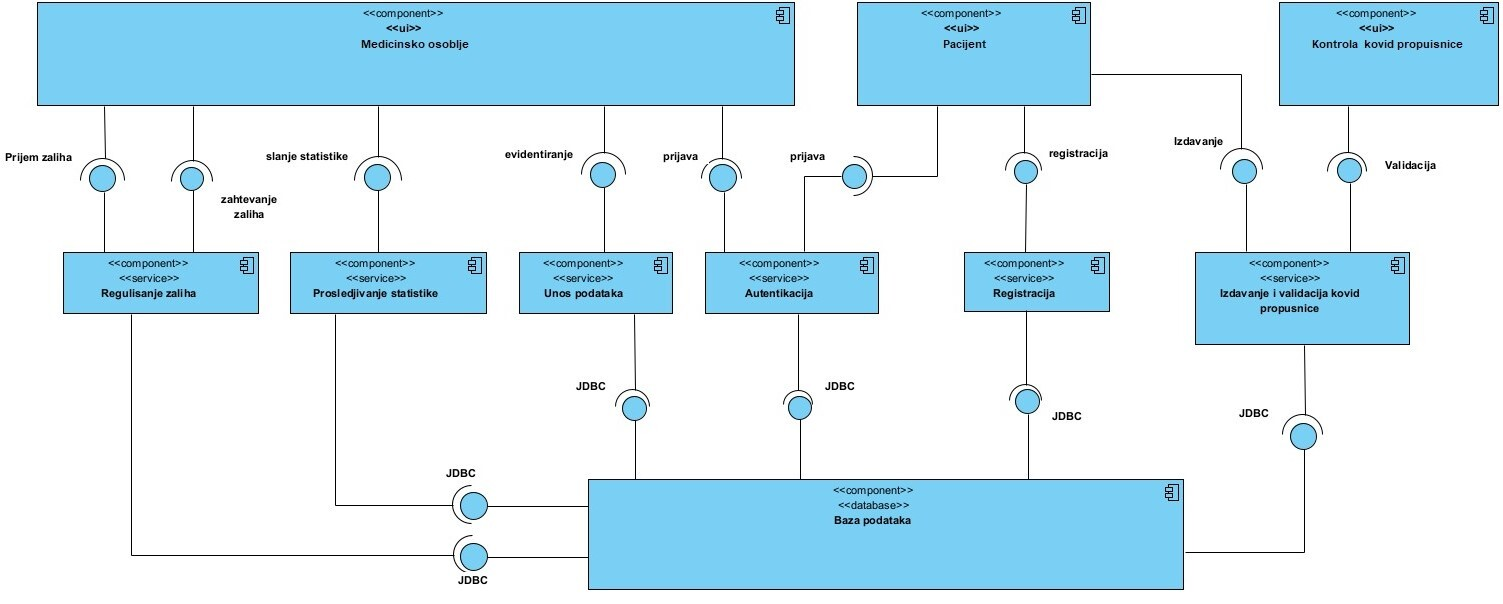
\includegraphics[scale=0.65]{Dijagram_komponenti}
\caption{Dijagram komponenti - softverska arhitektura}
\label{slk:komponente}
\end{figure}

Informacioni sistem je podeljen na server baze podataka i aplikacioni server koji komuniciraju pomoću TCP/IP protokola. Na serveru baze podataka se nalazi MySQL okruženje i baza sadrži tri sheme: Korisnici, Statistika i Ambulanta. Na aplikacionom serveru se koristi JSP server Tomcat 8 Catalina Servlet 3.1 i na njemu se izvršava aplikacija kovid\_centar.war. Aplikacija, između ostalog, implementira komponentu Evidentiranje. Konfiguracioni fajl aplikacije je web.xml. Deo aplikacije korisnicki\_servis1.jar implementira komponentu Korisnik - medicinsko osoblje, deo korisnicki\_servis2.jar implementira komponentu Korisnik - osoba, a deo korisnicki\_servis3.jar implementira komponentu Korisnik - ministarstvo. Aplikacija koristi biblioteku web\_tool\_lib.jar. Na Slici \ref{slk:isporucivanje} je prikazan dijagram isporučivanja sistema.

\begin{figure}[H]
\centering
\includegraphics[scale=0.4]{DijagramIsporucivanja}
\caption{Dijagram isporucivanja - softverska arhitektura}
\label{slk:isporucivanje}
\end{figure}




\end{document}
